%%%%%%%%%%%%%%%%%%%%%%%%%%%%%%%%%%%%%%%%%%%%%%%%%%%
%
%  New template code for TAMU Theses and Dissertations starting Fall 2012.  
%  For more info about this template or the 
%  TAMU LaTeX User's Group, see http://www.howdy.me/.
%
%  Author: Wendy Lynn Turner 
%
%%%%%%%%%%%%%%%%%%%%%%%%%%%%%%%%%%%%%%%%%%%%%%%%%%%

% TODO:
% Move to top margin: pg. ii, iii, iv, ix, 1, 7, 14, 26, 35, 42, 44

\documentclass[12pt]{report}
\renewcommand{\familydefault}{\rmdefault}
\usepackage[latin9]{inputenc}
\usepackage[letterpaper]{geometry}
\geometry{verbose,tmargin=1.25in,bmargin=1.25in,lmargin=1.4in,rmargin=1.15in}
\pagestyle{plain}
\usepackage[doublespacing]{setspace}
\usepackage{tocloft}
\usepackage[rm, tiny,center, compact]{titlesec}
\usepackage{indentfirst}
\usepackage{epstopdf}
\usepackage{graphicx,float,wrapfig}
\usepackage{etoolbox}
\usepackage{tocvsec2}
\usepackage[titletoc]{appendix}
\usepackage{appendix}
\usepackage{tamuconfig}
\usepackage[stable]{footmisc}
\usepackage[font=singlespacing]{caption}

\usepackage{amsmath}
\usepackage[noend]{algpseudocode}
\usepackage{algorithm}
\DeclareMathOperator{\pContact}{pContact}
\DeclareMathOperator{\pLocation}{pContact}
\DeclareMathOperator{\pTimeZone}{pTimeZone}
\DeclareMathOperator{\pStrangers}{pStrangers}
\DeclareMathOperator{\edges}{edges}
\DeclareMathOperator{\actEdges}{actEdges}
\DeclareMathOperator{\median}{median}
\DeclareMathOperator{\PLE}{PLE}
\DeclareMathOperator{\LCR}{LCR}
\DeclareMathOperator{\FriendLoc}{FriendLoc}
\DeclareMathOperator{\Backstrom}{Facebook}
\DeclareMathOperator{\p}{p}
\DeclareMathOperator{\haversin}{haversin}
\DeclareMathOperator{\Err}{Err}
\DeclareMathOperator{\AED}{AED}
\DeclareMathOperator{\ACC}{ACC}
\DeclareMathOperator{\quantile}{quantile}
\DeclareMathOperator*{\argmax}{arg\,max}
\renewcommand{\algorithmicthen}{}

\algnewcommand\algorithmicinput{\textbf{Input:}}
\algnewcommand\Input{\item[\algorithmicinput]}
\algnewcommand\algorithmicoutput{\textbf{Output:}}
\algnewcommand\Output{\item[\algorithmicoutput]}
\algnewcommand\algorithmiccontinue{\textbf{continue}}
\algnewcommand\Continue{\algorithmiccontinue}

\algdef{SE}[FOR]{ForEach}{EndFor}[1]{\algorithmicfor\ #1\ }{\algorithmicend\ \algorithmicfor}

\hyphenation{Four-square}
\hyphenation{Face-book}

%\newcommand{\jam}[1]{\emph{#1}}
%\newcommand{\jam}[1]{}
\newcommand{\temp}[1]{#1}
\newcommand{\flchap}[1]{\chapter{\uppercase{#1}}}
\newcommand{\flsec}[1]{\section{#1}}

\newcommand\blfootnote[1]{%
  \begingroup
  \renewcommand\thefootnote{}\footnote{#1}%
  \addtocounter{footnote}{-1}%
  \endgroup
}

% Hyperref setup below.  You should be able to get away with using uncommenting just the first line.
\usepackage[hidelinks]{hyperref}

% if \usepackage[hidelinks]{hyperref} doesn't work try this.
% \usepackage{hyperref}  % Hidelinks is an option that removes link visiability.  TAMU Thesis Offices prefers to not see the links. But often doesn't work.  
% 
% \hypersetup{
%     colorlinks=true,
%     linkcolor=black,
%     citecolor=black,
%     filecolor=black,
%     urlcolor=black,
% }
%%%%%%%  End of hyperref setup.  One of these two options should work, but my motto with hyperref is when in doubt, comment it out!

% attempt to single-space sections
\usepackage{tocloft}
\renewcommand{\cftsecafterpnum}{\vskip0.5\baselineskip}
\renewcommand{\cftsubsecafterpnum}{\vskip0.5\baselineskip}
\renewcommand{\cftsubsubsecafterpnum}{\vskip0.5\baselineskip}

\begin{document}
%mucking with floats by Jeff
\renewcommand\floatpagefraction{.9}
\renewcommand\textfraction{.1}

\renewcommand{\tamumanuscripttitle}{Location Prediction in Social Media Based
on Tie Strength}
\renewcommand{\tamupapertype}{Thesis}
\renewcommand{\tamufullname}{Jeffrey Allen McGee}
\renewcommand{\tamudegree}{Master of Science}
\renewcommand{\tamuchairone}{James Caverlee}
% Uncomment out the next line if you have co-chairs.  You will also need to edit the titlepage.tex file.
%\newcommand{\tamuchairtwo}{Additional Chair Name}
\renewcommand{\tamumemberone}{Frank Shipman}
\newcommand{\tamumembertwo}{Daniel Sui}
\renewcommand{\tamudepthead}{Hank Walker}
\renewcommand{\tamugradmonth}{May}
\renewcommand{\tamugradyear}{2013}
\renewcommand{\tamudepartment}{Computer Science}

% fix spacing in bibliography
\let\oldbibitem\bibitem
\renewcommand{\bibitem}{\setlength{\itemsep}{0pt}\oldbibitem}

% added by Jeff to split between thesis and www paper
\newcommand*{\THESIS}{}%

%%%%%%%%%%%%%%%%%%%%%%%%%%%%%%%%%%%%%%%%%%%%%%%%%%%
%
%  New template code for TAMU Theses and Dissertations starting Fall 2012.  
%  For more info about this template or the 
%  TAMU LaTeX User's Group, see http://www.howdy.me/.
%
%  Author: Wendy Lynn Turner 
%	 Version 1.0 
%  Last updated 8/5/2012
%
%%%%%%%%%%%%%%%%%%%%%%%%%%%%%%%%%%%%%%%%%%%%%%%%%%%

%%%%%%%%%%%%%%%%%%%%%%%%%%%%%% 
%% TITLE PAGE
%% The values get updated automatically.  Please do not make changes to this file other than adding/deleting committee members where necessary.
%%%%%%%%%%%%%%%%%%%%%%%%%%%%%%

\providecommand{\tabularnewline}{\\}



\begin{titlepage}
\begin{center}
\MakeUppercase{\tamumanuscripttitle}
\vspace{4em}

A \tamupapertype

by

\MakeUppercase{\tamufullname}

\vspace{4em}

\begin{singlespace}

Submitted to the Office of Graduate Studies of \\
Texas A\&M University \\

in partial fulfillment of the requirements for the degree of \\
\end{singlespace}

\MakeUppercase{\tamudegree}
\par\end{center}
\vspace{2em}
\begin{singlespace}
\begin{tabular}{ll}
Approved by: & \tabularnewline
& \cr
% If you have Co-Chairs comment out the 'Chair of Committee' line below and uncomment the 'Co-Chairs of Committee' line.
Chair of Committee, & \tamuchairone\tabularnewline
%Co-Chairs of Committee, & \tamuchairone\tabularnewline & \tamuchairtwo\tabularnewline
Committee Members, & \tamumemberone\tabularnewline
 & \tamumembertwo\tabularnewline
Department Head, & \tamudepthead\tabularnewline

\end{tabular}
\end{singlespace}
\vspace{4em}

\begin{center}
\tamugradmonth \hspace{2pt} \tamugradyear

\vspace{3em}

Major Subject: \tamudepartment \par
\vspace{3em}
Copyright \tamugradyear \hspace{.5em}\tamufullname 
\par\end{center}
\end{titlepage}
\pagebreak{}




 % This is simply a file that formats and adds your titlepage, please do not edit this unless you have a specific need. .
%%%%%%%%%%%%%%%%%%%%%%%%%%%%%%%%%%%%%%%%%%%%%%%%%%%
%
%  New template code for TAMU Theses and Dissertations starting Fall 2012.
%  For more info about this template or the
%  TAMU LaTeX User's Group, see http://www.howdy.me/.
%
%  Author: Wendy Lynn Turner
%	 Version 1.0
%  Last updated 8/5/2012
%
%%%%%%%%%%%%%%%%%%%%%%%%%%%%%%%%%%%%%%%%%%%%%%%%%%%
%%%%%%%%%%%%%%%%%%%%%%%%%%%%%%%%%%%%%%%%%%%%%%%%%%%%%%%%%%%%%%%%%%%%%
%%                           ABSTRACT
%%%%%%%%%%%%%%%%%%%%%%%%%%%%%%%%%%%%%%%%%%%%%%%%%%%%%%%%%%%%%%%%%%%%%

\chapter*{ABSTRACT}
\addcontentsline{toc}{chapter}{ABSTRACT} % Needs to be set to part, so the TOC doesnt add 'CHAPTER ' prefix in the TOC.

\pagestyle{plain} % No headers, just page numbers
\pagenumbering{roman} % Roman numerals
\setcounter{page}{2}

\indent We propose a novel network-based approach for location estimation in social
media that integrates evidence of the \textit{social tie strength} between
users for improved location estimation.
%
Concretely, we propose a location
estimator -- FriendlyLocation -- that leverages the relationship between the
strength of the tie between a pair of users, and the distance between the pair.
%
Based on an examination of over 100 million geo-encoded tweets and 73 million
Twitter user profiles, we identify several factors such as the
number of followers and how the users interact that can strongly reveal the
distance between a pair of users.
%
We use these factors to train a decision
tree to distinguish between pairs of users who are likely to live nearby and pairs of
users who are likely to live in different areas.
%
We use the results of this decision tree as the input to a maximum likelihood
estimator to predict a user's location.
We find that this proposed method significantly improves the results of
location estimation relative to a state-of-the-art technique.
Our system reduces the average error distance for 80\% of Twitter users from 40
miles to 21 miles using only information from the user's friends and
friends-of-friends,  which has great significance for augmenting traditional
social media and enriching location-based services with more refined and
accurate location estimates.

\pagebreak{}

%%%%%%%%%%%%%%%%%%%%%%%%%%%%%%%%%%%%%%%%%%%%%%%%%%%
%
%  New template code for TAMU Theses and Dissertations starting Fall 2012.  
%  For more info about this template or the 
%  TAMU LaTeX User's Group, see http://www.howdy.me/.
%
%  Author: Wendy Lynn Turner 
%	 Version 1.0 
%  Last updated 8/5/2012
%
%%%%%%%%%%%%%%%%%%%%%%%%%%%%%%%%%%%%%%%%%%%%%%%%%%%

%%%%%%%%%%%%%%%%%%%%%%%%%%%%%%%%%%%%%%%%%%%%%%%%%%%%%%%%%%%%%%%%%%%%%%
%%                           DEDICATION
%%%%%%%%%%%%%%%%%%%%%%%%%%%%%%%%%%%%%%%%%%%%%%%%%%%%%%%%%%%%%%%%%%%%%
\chapter*{DEDICATION}
\addcontentsline{toc}{chapter}{DEDICATION}  % Needs to be set to part, so the TOC doesnt add 'CHAPTER ' prefix in the TOC.



\indent This is an optional page.  Lorem ipsum dolor sit amet, consectetur adipiscing elit. Integer lectus quam, condimentum quis bibendum eu, sollicitudin eget lacus. Praesent non sodales odio. Class aptent taciti sociosqu ad litora torquent per conubia nostra, per inceptos himenaeos. Nulla ac luctus sapien. Morbi cursus sapien eget lorem fermentum hendrerit. Nam ac erat dui, in cursus velit. Vivamus hendrerit porttitor nisi, ut porttitor lorem volutpat eget. In ligula ligula, euismod ut condimentum sit amet, pulvinar sit amet diam. Pellentesque interdum, ipsum ullamcorper consequat dignissim, sem arcu egestas mauris, vitae interdum sem tortor ut ante. Nunc blandit laoreet nisi, non rutrum lorem hendrerit quis. Cras nunc diam, convallis et feugiat at, auctor id libero. Nunc facilisis massa eu eros imperdiet vestibulum. Vestibulum ante ipsum primis in faucibus orci luctus et ultrices posuere cubilia Curae; Donec non velit vitae tortor blandit semper.

Etiam vitae dolor nulla. Ut eros odio, rhoncus eget placerat vitae, elementum ac ante. Proin vitae odio eu nisl pharetra mattis. Pellentesque habitant morbi tristique senectus et netus et malesuada fames ac turpis egestas. Phasellus fermentum lacus consectetur neque consequat ullamcorper. Cras blandit urna non dui consequat molestie. Curabitur viverra nibh at nisi semper faucibus. Nam egestas mauris a enim dignissim nec consectetur tortor rutrum. Mauris at nisi in est luctus congue ut mattis est. Ut pretium, mi quis elementum cursus, ante eros suscipit ligula, ut porttitor elit leo sed turpis. Nam sed dui ligula.


\pagebreak{}

%%%%%%%%%%%%%%%%%%%%%%%%%%%%%%%%%%%%%%%%%%%%%%%%%%%
%
%  New template code for TAMU Theses and Dissertations starting Fall 2012.  
%  For more info about this template or the 
%  TAMU LaTeX User's Group, see http://www.howdy.me/.
%
%  Author: Wendy Lynn Turner 
%	 Version 1.0 
%  Last updated 8/5/2012
%
%%%%%%%%%%%%%%%%%%%%%%%%%%%%%%%%%%%%%%%%%%%%%%%%%%%


%%%%%%%%%%%%%%%%%%%%%%%%%%%%%%%%%%%%%%%%%%%%%%%%%%%%%%%%%%%%%%%%%%%%%%
%%                           ACKNOWLEDGEMENTS
%%%%%%%%%%%%%%%%%%%%%%%%%%%%%%%%%%%%%%%%%%%%%%%%%%%%%%%%%%%%%%%%%%%%%
\chapter*{ACKNOWLEDGEMENTS}
\addcontentsline{toc}{chapter}{ACKNOWLEDGEMENTS}  % Needs to be set to part, so the TOC doesnt add 'CHAPTER ' prefix in the TOC.


\indent Lorem ipsum dolor sit amet, consectetur adipiscing elit. Integer lectus quam, condimentum quis bibendum eu, sollicitudin eget lacus. Praesent non sodales odio. Class aptent taciti sociosqu ad litora torquent per conubia nostra, per inceptos himenaeos. Nulla ac luctus sapien. Morbi cursus sapien eget lorem fermentum hendrerit. Nam ac erat dui, in cursus velit. Vivamus hendrerit porttitor nisi, ut porttitor lorem volutpat eget. In ligula ligula, euismod ut condimentum sit amet, pulvinar sit amet diam. Pellentesque interdum, ipsum ullamcorper consequat dignissim, sem arcu egestas mauris, vitae interdum sem tortor ut ante. Nunc blandit laoreet nisi, non rutrum lorem hendrerit quis. Cras nunc diam, convallis et feugiat at, auctor id libero. Nunc facilisis massa eu eros imperdiet vestibulum. Vestibulum ante ipsum primis in faucibus orci luctus et ultrices posuere cubilia Curae; Donec non velit vitae tortor blandit semper.

Etiam vitae dolor nulla. Ut eros odio, rhoncus eget placerat vitae, elementum ac ante. Proin vitae odio eu nisl pharetra mattis. Pellentesque habitant morbi tristique senectus et netus et malesuada fames ac turpis egestas. Phasellus fermentum lacus consectetur neque consequat ullamcorper. Cras blandit urna non dui consequat molestie. Curabitur viverra nibh at nisi semper faucibus. Nam egestas mauris a enim dignissim nec consectetur tortor rutrum. Mauris at nisi in est luctus congue ut mattis est. Ut pretium, mi quis elementum cursus, ante eros suscipit ligula, ut porttitor elit leo sed turpis. Nam sed dui ligula.


\pagebreak{}
%%%%%%%%%%%%%%%%%%%%%%%%%%%%%%%%%%%%%%%%%%%%%%%%%%%%
%
%  New template code for TAMU Theses and Dissertations starting Fall 2012.  
%  For more info about this template or the 
%  TAMU LaTeX User's Group, see http://www.howdy.me/.
%
%  Author: Wendy Lynn Turner 
%	 Version 1.0 
%  Last updated 8/5/2012
%
%%%%%%%%%%%%%%%%%%%%%%%%%%%%%%%%%%%%%%%%%%%%%%%%%%%

%%%%%%%%%%%%%%%%%%%%%%%%%%%%%%%%%%%%%%%%%%%%%%%%%%%%%%%%%%%%%%%%%%%%%%
%%                           NOMENCLATURE
%%%%%%%%%%%%%%%%%%%%%%%%%%%%%%%%%%%%%%%%%%%%%%%%%%%%%%%%%%%%%%%%%%%%%

\chapter*{NOMENCLATURE}
\addcontentsline{toc}{chapter}{NOMENCLATURE}  % Needs to be set to part, so the TOC doesnt add 'CHAPTER ' prefix in the TOC.

\begin{tabular}{ll}
B/CS  & Bryan/College Station\tabularnewline
HSUS & Humane Society of the United States\tabularnewline
P & Pressure\tabularnewline
T  & Time\tabularnewline
TVA & Tennessee Valley Authority\tabularnewline
TxDOT \hfill{}\hfill{}\hfill{}\hfill{}\hfill{}\hfill{}\hfill{}\hfill{} & \multicolumn{1}{l}{Texas Department of Transportation}\tabularnewline
\end{tabular}

\vspace{2em}

This page is optional.

\pagebreak{}

%%%%%%%%%%%%%%%%%%%%%%%%%%%%%%%%%%%%%%%%%%%%%%%%%%%
%
%  New template code for TAMU Theses and Dissertations starting Fall 2012.  
%  For more info about this template or the 
%  TAMU LaTeX User's Group, see http://www.howdy.me/.
%
%  Author: Wendy Lynn Turner 
%	 Version 1.4
%  Last updated 1/27/2013
%
%%%%%%%%%%%%%%%%%%%%%%%%%%%%%%%%%%%%%%%%%%%%%%%%%%%
%%%%%%%%%%%%%%%%%%%%%%%%%%%%%%%%%%%%%%%%%%%%%%%%%%%%%%%%%%%%%%%%%%%%%%
%%       TABLE OF CONTENTS
%%%%%%%%%%%%%%%%%%%%%%%%%%%%%%%%%%%%%%%%%%%%%%%%%%%%%%%%%%%%%%%%%%%%%
\phantomsection
\addcontentsline{toc}{chapter}{TABLE OF CONTENTS}  

\begin{singlespace}
\renewcommand\contentsname{\normalfont} {\centerline{TABLE OF CONTENTS}}

%\setcounter{tocdepth}{4} % This puts \subsubsection[]{×} in your List of Tables.  The default is 3.


%%%%%%%%%%%%%  Adds Page above the page number in TOC
\setlength{\cftaftertoctitleskip}{1em}
\renewcommand{\cftaftertoctitle}{%
\hfill{\normalfont {Page}\par}}



\tableofcontents

\end{singlespace}

\pagebreak{}

%%%%%%%%%%%%%%%%%%%%%%%%%%%%%%%%%%%%%%%%%%%%%%%%%%%%%%%%%%%%%%%%%%%%%%
%%                           LIST OF FIGURES
%%%%%%%%%%%%%%%%%%%%%%%%%%%%%%%%%%%%%%%%%%%%%%%%%%%%%%%%%%%%%%%%%%%%%

\phantomsection
\addcontentsline{toc}{chapter}{LIST OF FIGURES}  

\renewcommand{\cftloftitlefont}{\center\normalfont\MakeUppercase}

\setlength{\cftbeforeloftitleskip}{-12pt} %% Positions the LOF title vertically to match the chapter titles
\renewcommand{\cftafterloftitleskip}{12pt}


\renewcommand{\cftafterloftitle}{%
\\[4em]\mbox{}\hspace{2pt}FIGURE\hfill{\normalfont Page}\vskip\baselineskip}

\begingroup


\begin{center}
\begin{singlespace}
%% These values make the lof table entries appear double spaced between.
\setlength{\cftbeforechapskip}{0.4cm}
\setlength{\cftbeforesecskip}{0.30cm}
\setlength{\cftbeforesubsecskip}{0.30cm}
\setlength{\cftbeforefigskip}{0.4cm}
\setlength{\cftbeforetabskip}{0.4cm} 

\listoffigures

\end{singlespace}
\end{center}

\pagebreak{}


%%%%%%%%%%%%%%%%%%%%%%%%%%%%%%%%%%%%%%%%%%%%%%%%%%%%%%%%%%%%%%%%%%%%%%
%%                           lIST OF TABLES
%%%%%%%%%%%%%%%%%%%%%%%%%%%%%%%%%%%%%%%%%%%%%%%%%%%%%%%%%%%%%%%%%%%%%%
%
\phantomsection
\addcontentsline{toc}{chapter}{LIST OF TABLES}  

\renewcommand{\cftlottitlefont}{\center\normalfont\MakeUppercase}

\setlength{\cftbeforelottitleskip}{-12pt} %% Positions the LOT title vertically to match the chapter titles

\renewcommand{\cftafterlottitleskip}{12pt}


\renewcommand{\cftafterlottitle}{%
\\[4em]\mbox{}\hspace{4pt}TABLE\hfill{\normalfont Page}\vskip\baselineskip}

\begin{center}
\begin{singlespace}

%% These values make the lot table entries appear double spaced between.
\setlength{\cftbeforechapskip}{0.4cm}
\setlength{\cftbeforesecskip}{0.30cm}
\setlength{\cftbeforesubsecskip}{0.30cm}
\setlength{\cftbeforefigskip}{0.4cm}
\setlength{\cftbeforetabskip}{0.4cm}

\listoftables 

\end{singlespace}
\end{center}
\endgroup
\pagebreak{}  % Need this for the pagenumbering to be correct. 
  % This is simply a file that formats and adds your toc, lof, and lot, please do not edit this unless you have a specific need. .

%\jam{too much space between subheadings in table of contents}

%\jam{sections should be title case or sentence case, not both}

%\jam{list of figures and tables contains full captions, not titles}

%\jam{fix citations for  ``Inferring the location of twitter messages based on
%    user relationships''}

\ifdefined\THESIS
    \pagestyle{plain} % No headers, just page numbers
    \pagenumbering{arabic} % Arabic numerals
    \setcounter{page}{1}
    \chapter{\uppercase {Introduction and Related Work}}
\else
\fi

\section{Introduction}

FIXME: rewrite this whole file


Online social networks are increasingly getting ``geographical.'' Millions of
online
social network users are voluntarily sharing their location through location
sharing
services like Foursquare, short text status updates
through real-time microblogs, and photos in online image hosts. This location
information is increasingly being
incorporated in social media for providing localized content, location-aware
recommendations, and other geo-spatial enabled services. The access to the
trails and connections among millions of social media users provides an
unprecedented opportunity to study the relationship between the geographical
properties of social media users and the social relations connecting them.

With high-quality geographic information, online services become more useful to
the local community.  Online services can bring to light discussions about what
the city council voted on last night.  Online services can identify, and react
to, the crowd of people gathering for the big football game.  Online services
can do a better job suggesting friends.  Online services can reconnect users
with the community that the users neglected when they started spending their
time online.

Geographic information is also useful for researchers.  In the past few years,
there has been growth in research into topics such as geographical user
clustering and location-based social networks.  As the accuracy of geographic
information improves, it will open up new research opportunities.

In this paper, we investigate the interplay of distance and tie strength
through an examination of FIXME million geo-encoded tweets and FIXME million user
profiles collected from Twitter. Concretely, we investigate the relationship
between the strength of the tie between a pair of users and the distance
between the pair.  We identify several factors -- including following,
mentioning, and actively engaging in conversations with another user -- that
can strongly reveal the distance between a pair of users.

FIXME: bimodal? The US data is bimodal, but the world data is not. Should we
discuss this? Most other related papers only look at inside US.

We find a bimodal distribution in the distance between Twitter users, with one
peak around 10 miles from people who live nearby, and another peak around 2500
miles, further validating Twitter's use as both a social network (with
geographically nearby friends) and as a news distribution network (with very
distant relationships).  Figure~\ref{fig:EdgeTypes} gives a preview of this
bimodal distribution for four basic types of relationships.  The red curve
represents a strong, reciprocal friendship whereas the cyan line represents a
relatively weak relationship. The red curve has more users at a distance of ten
miles than the cyan line, indicating that reciprocal friendships are more
likely to be local.

Based on these findings, we propose and evaluate a framework for predicting
location for users based on an analysis of the user's social network,
which has great significance for augmenting traditional social media and
enriching location-based services with more refined and accurate location
estimates.  FriendlyLocation correctly locates FIXME\% of users within 25 miles.

\section{Related Work}

%FIXME: Mr. Cheng wrote some of this.

The study of geographical properties of online social media users has drawn
intensive attention in recent years.  Characterizing network properties in
relation to local geography has been studied in \cite{yardi2010tweeting}.
Lindqvist \cite{lindqvist2011m} analyzed how and why people use location
sharing services, and discussed the privacy issues related to location sharing
services.

Scellato et al. \cite{scellato2011socio} used data from three location based
social networks to investigate the relationship between distance and location,
and they show that connections are not purely caused by geographical or social
factors.  They investigated two random models where they shuffle the user
locations and another where they shuffle the social connections and investigate
what happens to the user location.  They show that if a user has more
connections, then their friends tend to be further away.  They also found that
longer connections are equally likely to be part of a social triangle as
shorter connections.

We know of two previous systems that attempted to estimate the location of
users on social networking sites.  In the first, Facebook researchers analyzed
the physical distance between Facebook users' social relations and utilized the
locations of a user's friends' to predict the user's geographical location
\cite{backstrom2010find}.  They picked users who entered their street address
in the location field of their profile and used this to predict the location of
their friends using maximum likelihood estimation.  However, the information
they used is generally not available outside of Facebook, since people rarely
make their street address public.  Cheng et al. \cite{cheng2010you} propose a
content-based system for locating users on Twitter. They find words that are
highly concentrated in specific regions and build a model to calculate the
probability that a user lives at a location.

FIXME: add new papers here - especially the twitter ones

Gilbert \cite{gilbert2009predicting} shows how the strength of a tie can be
predicted by interaction patterns.  They had volunteers rate the strength of
several friendships and then analyzed the activity between the users can
predict the strength of the friendship.  We argue that tie strength is also
correlated with physical proximity.

There has also been some research into specific aspects of Twitter that is
relevant to our work.  User behavior with regard to the location field in
Twitter user profiles has been studied in \cite{hecht2011tweets}.  One of the
early investigations into Twitter usage by Java \cite{java2007we} showed that
people use twitter for chatter, conversations, sharing information, and
reporting news.  This mixture of uses fits well with the bimodal distribution
of friends and followers that we propose.

Finally, Cranshaw et al. \cite{cranshaw2010bridging} solved the inverse of the
problem we are investigating: they predicted the existence of a social network
tie given precise location information from laptops and cell phones. They used
a collection of features of when users are co-located.  Together, these efforts
have begun to lay a foundation for the study \textit{geo-social media}.


\ifdefined\THESIS
    \chapter{\uppercase {Data Collection}}

\else
    \section{Data Collection}
\fi

\section{Definitions}

\jam{Talk about how geo-located users are different.}
\jam{Do cool stuff}

Before going into the details of the data collection, we first define a few
terms to simplify the process of explaining how the data was collected.
%
Figure~\ref{fig:Terms} shows a social graph and uses most of the terms defined
in this section.
%
\textbf{Contacts} are defined to be the set of a user's friends, followers, and
people who a user mentioned in her tweets (i.e., people the user speaks to).
%
Since Twitter does not provide a mechanism to determine who mentioned a given
user, only one-directional conversation is considered.
%
In some blogging platforms, such as Tumblr, it is relatively easy to find the
communication edges that point back toward a user.
%
In those platforms, it would be fairly straightforward to use that information
in location prediction.

\begin{figure}[tbh]
\centering
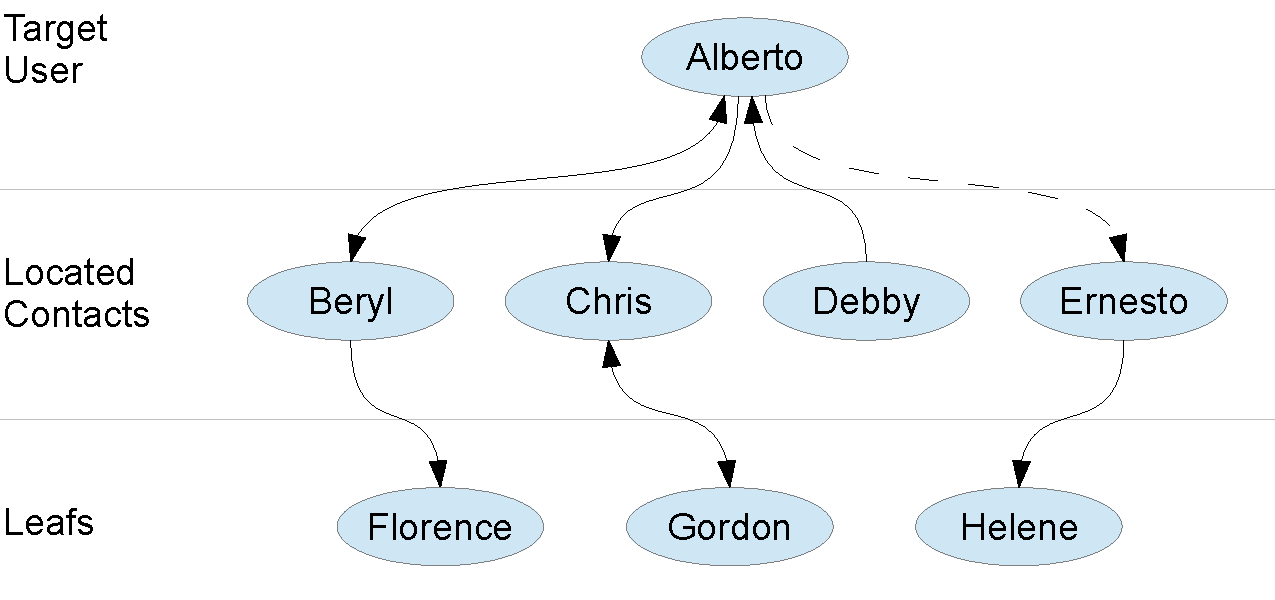
\includegraphics[width=\linewidth]{figures/terms.pdf}
\caption{
A small sample social graph for illustrating definitions used in this paper.
Alberto adds location information to his tweets.
Beryl is a reciprocal friend of Alberto, Chris is just a friend since Alberto
follows Chris, Debby is just a follower, and Ernesto is just mentioned.
The line to Ernesto is dashed to show that there is no friend/follow
relationship between Alberto and Ernesto.
The other arrows show who follows whom.
}
\label{fig:Terms}
\end{figure}

Any given contact can be categorized into precisely one of these four disjoint
sets:
\begin{description}
\item[reciprocal friend] The target user follows this user and is followed
    back.
\item[just friend] The target user follows this user and is not followed
    back.
\item[just follower] The target user is followed by this user, but does
    not follow them.
\item[just mentioned] The users do not follow each other, but the target
    user mentioned the name of the other user in a tweet.
\end{description}

Our crawler starts from a set of seed users and goes two steps out on the
social graph.
%
We created labels for the seed users and each of the steps along the way:

\begin{description}
\item[geo-located users] These users choose to use Twitter's location sharing
    features, which means that we have precise latitude and longitude
    coordinates for their location.
\item[target users] These are a randomly chosen subset of the geo-located users
    who have at least one contact.
\item[geocoder calibration users] These are geo-located users who filled out their
    location field with a location we could decode, but were not selected to be
    part of the target users. They are used to differentiate between
    high-quality locations and low-quality locations that are likely to be
    wrong.
\item[located contacts] These are the 25 randomly chosen contacts of
    target users who have locations that we can decode.
\item[leaves] These are at most 100 of the contacts of the located contacts.
    When we selected leaves, we excluded the target users from the contacts so
    that the distances to contacts would be independent from the distances to
    leaves.
\end{description}


\section{Data Collection}
To investigate how social relation and geographical distance between the
relations correlate, we sample a dataset from Twitter.
%
Our analysis and prediction is based on data collected from Twitter during
May, June, and July of 2012.

We built a crawler to find these contacts for users who used Twitter's Location
Feature to disclose their location.
The crawler sampled over one hundred million geo-coded tweets by monitoring
Twitter's public streaming API for all of May 2012.
% 118,464,320 lines including keepalive newlines and non-status messages.
We kept the tweets from the users who posted at least three tweets, which left
us with 1758101 Twitter users.
%
For each of these users with geo-coded tweets, we use the median latitude and
median longitude of the locations of the user's tweets as an approximation of
her home location.
%
Some Twitter accounts, such as accounts that posted jobs, would
move around faster than a human could possibly move.
%
To account for this, the crawler calculated the distance between each tweet and
the user's home location.
%
The crawler ignored users if the median distance from their tweets to their
home location is greater than 50 miles.
%
This only removed 3.4\% of the geo-located users.
%
We also removed an additional 2.9\% of the geo-located users who did not have
any contacts with locations we could decode, which left us with 1.6 million
Twitter users with a known location.
%
We randomly selected 249,584 of these users for analysis and experimentation.
\footnote{We originally selected 250,000 users, but had to remove 416 of them.
These users had contacts with locations, but none of their contacts had
meaningful locations.}
%
Almost all of the experiments in this paper are based on these target
users.

%To enable parallelization, we divided those users into 100 groups based on
%the two least significant digits in their Twitter user id, and randomly selected
%2500 users from each of the groups.

% distribution of the contacts
%     med  avg      std
%rfrd 62.0 132.7148 278.394
%jfol 35.0 143.4844 456.629
%jfrd 78.0 153.5700 241.222
%jats  5.0   7.0764   8.060

For all of the target users, the crawler used Twitter's API to download
the users' 100 most recent tweets, a list of friend ids, and a list of follower ids.
%
Most of the target users had plenty of contacts of each of the four types.
%
The median number of reciprocal friends is 62, and the average is 132.
%
The average numbers are higher because the number of contacts a user has
follows a heavy-tailed distribution.
%
The medians for other types of contacts are 35 just followers, 78 just friends,
and 7 just mentioned.
%
If a user had over 25 contacts in any of the four types of contacts, the
crawler chose a random sample of 25 from each of the types of contacts, and
downloaded the profiles for up to 100 total contacts per target user.
%
From that 100, we randomly picked at most 25 contacts with locations we could
decode to be the located contacts. For those located contacts, we downloaded
their friends, followers, and tweets.
%
We finished this process by downloading up to 100 profiles of the contacts of
the contacts.
%
Since the Twitter social network graph has a large strongly connected
component, there are a significant number of users who are contacts or leafs for
more than one target user.
%
In the end, we collected just over 73 million Twitter user profiles.

\section{Geocoding}
We used Gisgraphy\footnote{\url{http://www.gisgraphy.com/}} to do geocoding.
%
Gisgraphy does full-text search on the
GeoNames\footnote{\url{http://www.geonames.org/}} database using Lucene.
%
Since it runs locally it is not limited to a certain number of queries per day.
%
Gisgraphy's geocoder returns ranked results based on a full text search
over millions of geographical features such as countries, cities, and schools.

The location field on a user's profile is just a text field that asks the user
to respond to ``Where in the world are you?''.
%
Responses vary from precise latitude and longitude coordinates entered
automatically by smartphone apps to jokes and nonsense.
%
Our system does some preprocessing before sending user-submitted locations to
the geocoder.
%
First, it uses a regular expression to find latitude and longitude coordinates,
which are treated as if they were a unique type of location returned by the
geocoder.
%
Occasionally, users would put two locations separated by a slash, dash or a
conjunction, and we pick the first one that we could decode.
%
If the geocoder did not return any results for a user, our system tried to
geocode both locations and returned the first location that the geocoder
understood.

Some locations are significantly more useful than others.
For example, even though Rhode Island and Montana are both states with around
one million people, Rhode Island is smaller, and as a result, much more useful
in estimating the location of a user.
To make the results of the geocoder more useful, we devised a method to
estimate the accuracy of a location returned by the geocoder.

\begin{table}[tb]
\centering
\caption{Example Median Location Errors (in miles).}
\begin{tabular}{l r r}
Location&Number of Users&Median Error\\ \hline
``Bronx''&438&4\\
``New York''&7483&175\\
``Pluto''&238&8272\\ \hline
\\
Place Type&Number of Users&Median Error\\ \hline
(latitude, longitude)&76552&3\\
A City&20914&6\\
A Hotel&1052&29\\
An Airport&410&258\\
A Stream&739&2373\\
\hline\end{tabular}
\label{tab:MedianLocErr}
\end{table}

Since we only selected a fraction of the 1.7 million users who posted tweets with
location information for location prediction and analysis, the remaining users
could be used for calibrating the geocoder.
%
894,617 of the users who posted geo-located tweets also filled in the
the free-response location field with something that the geocoder is able to
decode.
%
These users form the geocoder calibration group.

We can compare the results of the geocoder to the location of the geo-located
tweets for these users to quantify how accurate the geocoder is for certain
types of locations.
%
We define the \textbf{location error} to be the great circle distance between a
user's home location and the location returned from the geocoder:

\jam{Do we need the $i$ here?}
\[
e_i = |l^h_i - l^g_i|
\]

The location error for a user can vary from less than a mile to over ten
thousand miles.
%
We calculated the location error for each of the geo-located users selected for
evaluating the geocoder, and sorted the users by their location.
%
For the 17,370 locations that had at least three users, we calculated the median
location error for that location.
%
All the users who were at locations with only one or two users were grouped
according to the type of location returned by the geocoder.
%
We calculated the median error for each location type.
%
The median is more appropriate than the average or standard deviation because
those metrics are strongly affected by large outliers.
%
We choose to make the cutoff three because that is the smallest value where the
median is not just an average.
Table~\ref{tab:MedianLocErr} shows the median location error for a few example
locations and location types.

This gives us a method to estimate the quality of a coordinate returned by
Gisgraphy.
%
We define the \textbf{predicted location error (PLE)} for a given location to
be the median location error if it is one of the 17,370 locations that had
at least three users; otherwise, it is the median location error for the location's
type.
%
For example, one user had ``PDX,OR'' in his location field.
%
Gisgraphy identifies this as ``Portland International Airport''.
%
Since it is not one of the most common locations, its PLE is determined by its
place type to be 258 miles as seen in Table~\ref{tab:MedianLocErr}.
%
An airport is a bad location name since airports tend to have regional names
and people who report their location as an airport are likely to move around a
lot.

\newcommand{\geotuple}{{(l^g_i,p_i,t_i,e_i) \in T}}

We will now formally define predicted location error.
%
We treat the locationsreturned by the geocoder as a set of tuples $\geotuple$,
where $l^g_i$ is the latitude and longitude, $p_i$ is the id of the place, and
$t_i$ is the id of the type of place, and $e_i$ is the location error.

For notational convenience, we define a set of places $F$ that have at least
three users:
\jam{is there a better way to say this?}
\[
    F = \{ p_i \mid \geotuple \land |\{(l^g_j,p_j,t_j,e_j) \in T|p_i==p_j\}| \geq 3 \}
\]

This lets us define $PLE$ as a function of a place and type of place:
\[
    PLE(p,t) =
    \begin{cases}
        \median(\{e_i |\geotuple \land p_i=p\})  & p \in F \\
        \median(\{e_i |\geotuple \land t_i=t \land p_i \notin F\})  & p \notin F \\
    \end{cases}
\
\]

\begin{figure}[tb]
\centering
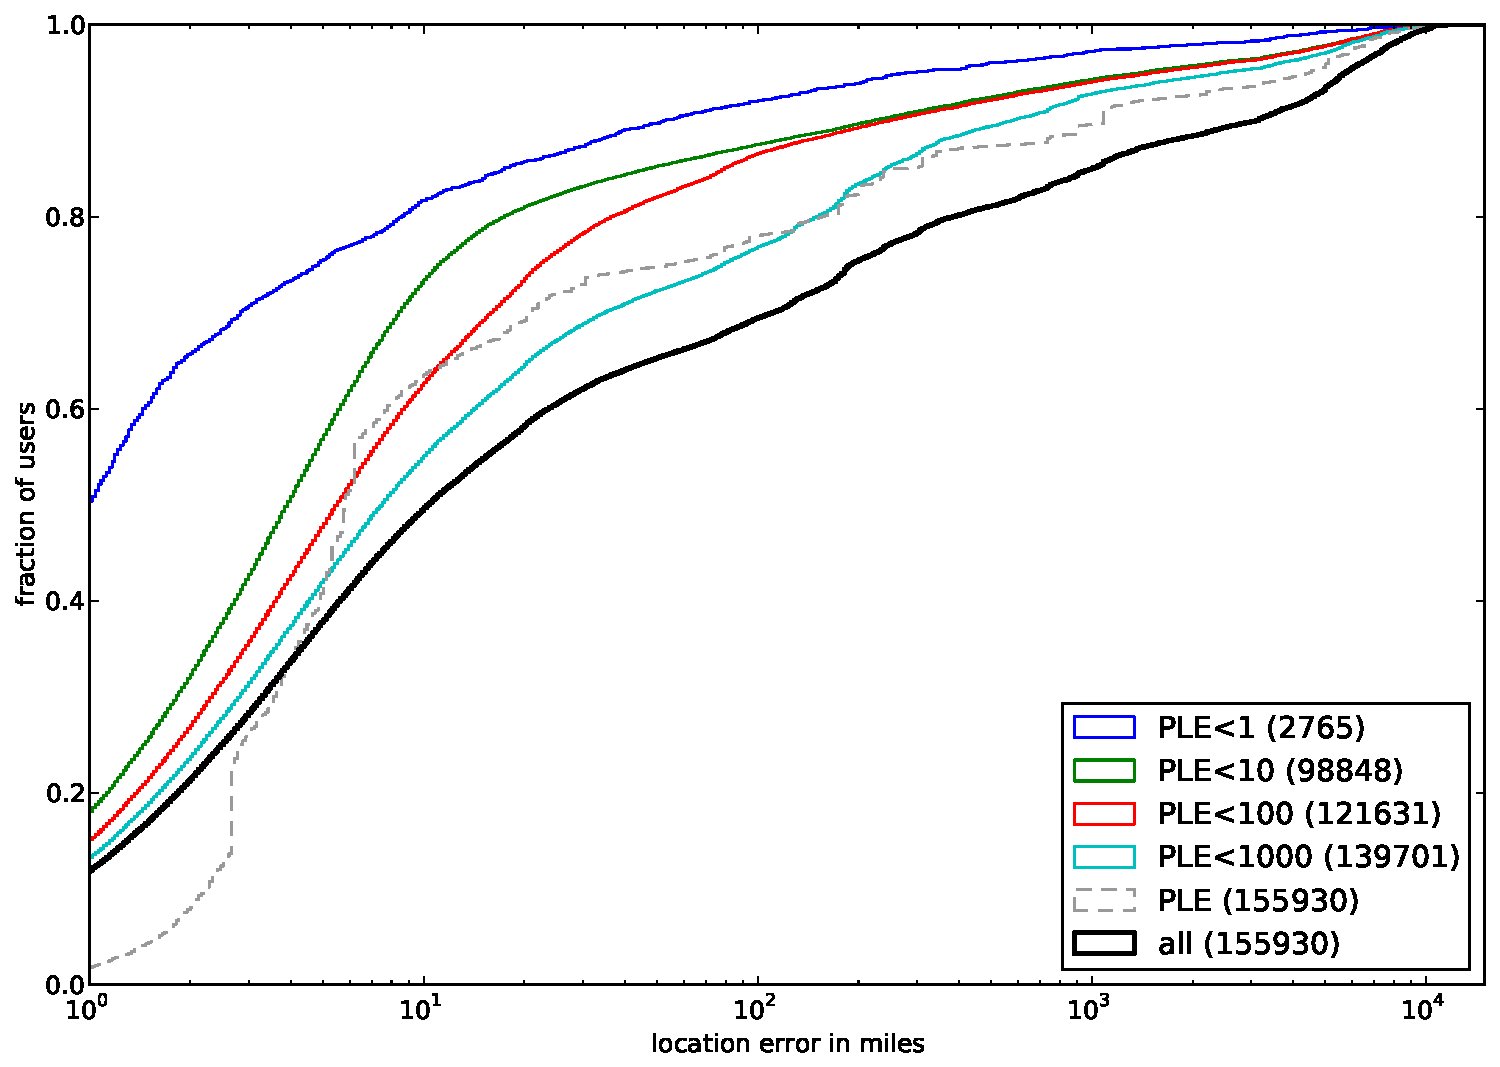
\includegraphics[width=\linewidth]{figures/mloc_mdist.pdf}
\caption{
Cumulative distribution function(CDF) of the distance between geo-located
users' tweets and their geocoded self-reported location.
%
The distances are split into bins based on the predicted location error(PLE).
%
The blue lines show that locations with a low PLE tend to be accurate, and
locations with a high PLE are rarely accurate.
%
The dotted line shows the values of the PLE for all the
users in this graph.
%
63\% of these users have a PLE less than 10 miles, and 90\% have a PLE
less than 1000.
}
\label{fig:DiffMlocMdist}
\end{figure}

The blue curves in Figure~\ref{fig:DiffMlocMdist} show a comparison of the PLE
and the actual location error for 155,930 of the target users (these are the
target users who also filled out the location field of their profile).
%
90\% of these users have a PLE that is less than 1000 miles.
%
85\% of the target users live within 1000 miles of the location returned by
the geocoder, but after removing only the 10\% of them who have a PLE greater
than 1000 miles, 93\% of the remaining users live within 1000 miles of the
location the geocoder returns.
%
In all of the future experiments, we treat locations with a PLE that is greater
than 1000 as if no location had been supplied.
%
This filters out worthless locations such as ``Pluto'', while keeping somewhat
vague, but still potentialy useful locations such as ``California''.


\chapter{\uppercase{Analysis of Distance to Contacts}}

Every user who has multiple contacts will have some contacts who are much
closer than others. In order to estimate the locations of users, we would like
to find out which users are most likely to live nearby.  In this section, we
investigate how various types of contacts correlate with proximity.
All of the analysis in this section was done on the contacts of 249584 geo-located users.
Contacts with a predicted location error that was greater than or equal to 1000
miles were filtered out.

\section{What type of contact is closest?}
\label{sec:EdgeTypes}

\begin{figure}[tb]
\centering
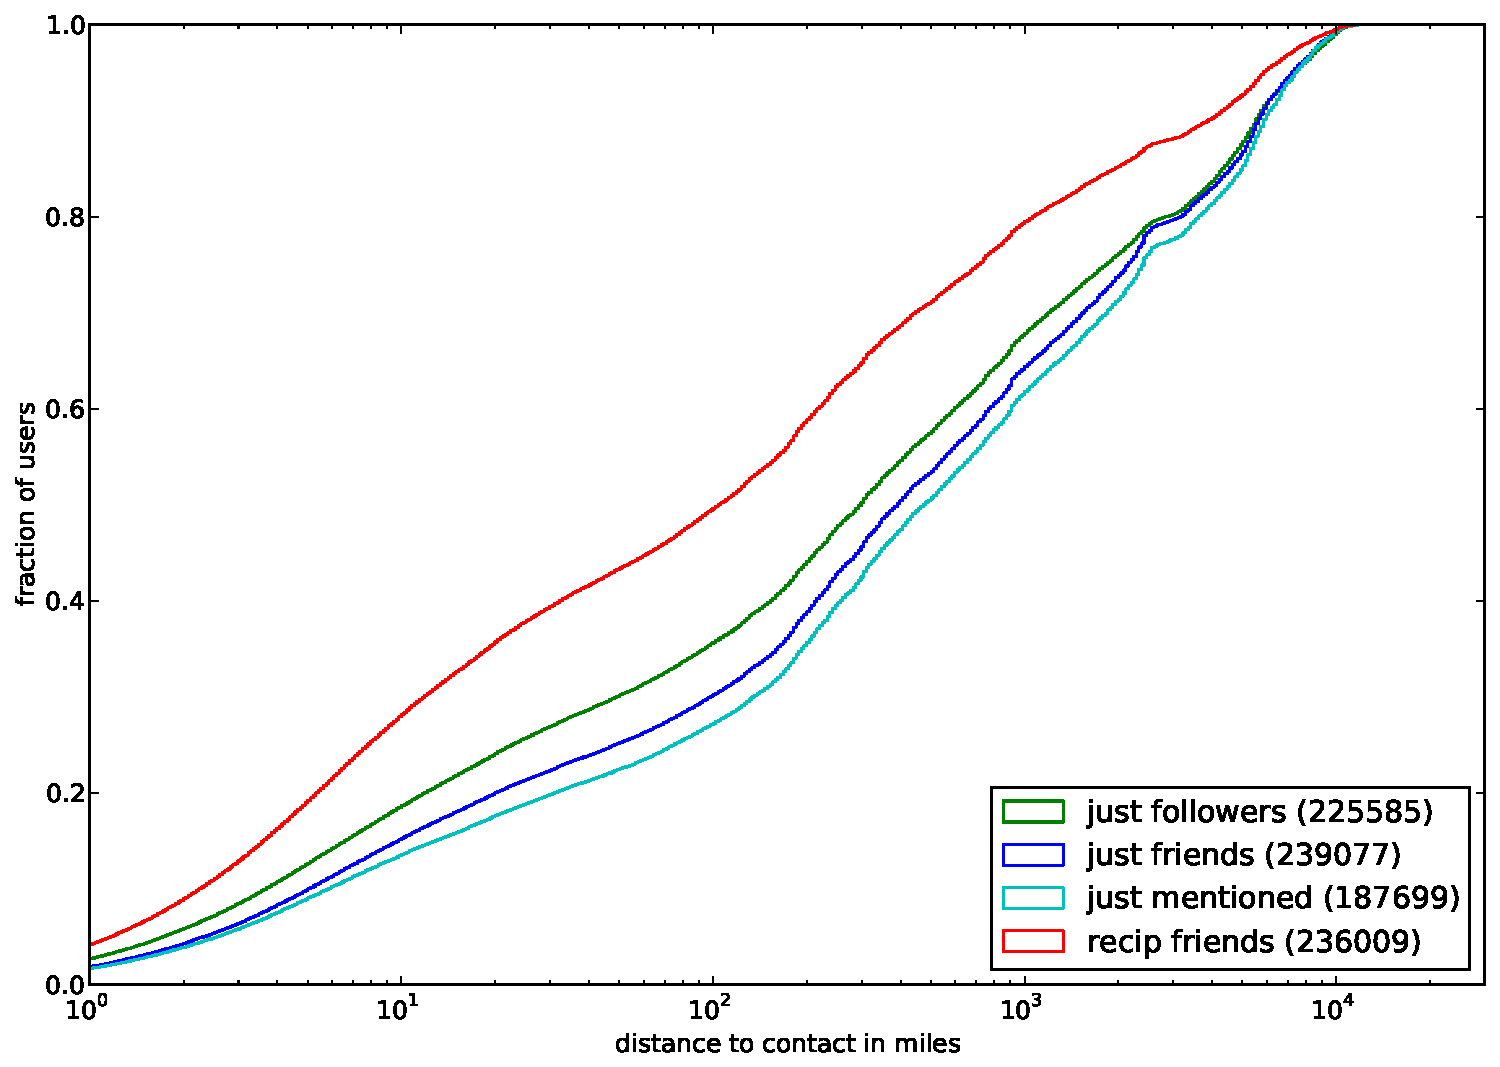
\includegraphics[width=\linewidth]{figures/edge_types_cuml.pdf}
\caption{
CDF of distance from geo-located users to users they have some contact
with.
}
\label{fig:EdgeTypesCum}
\end{figure}

Figure~\ref{fig:EdgeTypesCum} shows the cumulative distribution
function(CDF) of the distance between a geo-located user and several types of
contacts.
Distance is plotted on a logarithmic scale to show both local and
global effects.

In general, reciprocal friends are the closest, followed by followers, friends,
and finally users who are just mentioned.
37\% of reciprocal friends live within 25 miles while only 18\% of users
who are just mentioned live within that radius.
While it may seem that since being followed by someone and following someone
should be identical, they are not.
Celebrity and news accounts on Twitter often have large numbers of followers,
but they normally do not follow a large number of users.
Since the geo-located user was selected randomly, they are usually an average
user and not a celebrity.
If they follow someone, it might be a celebrity; however, if someone follows
them, it is probably someone who knows them.

\section{What is the distribution of contacts?}

\begin{figure}[tb]
\centering
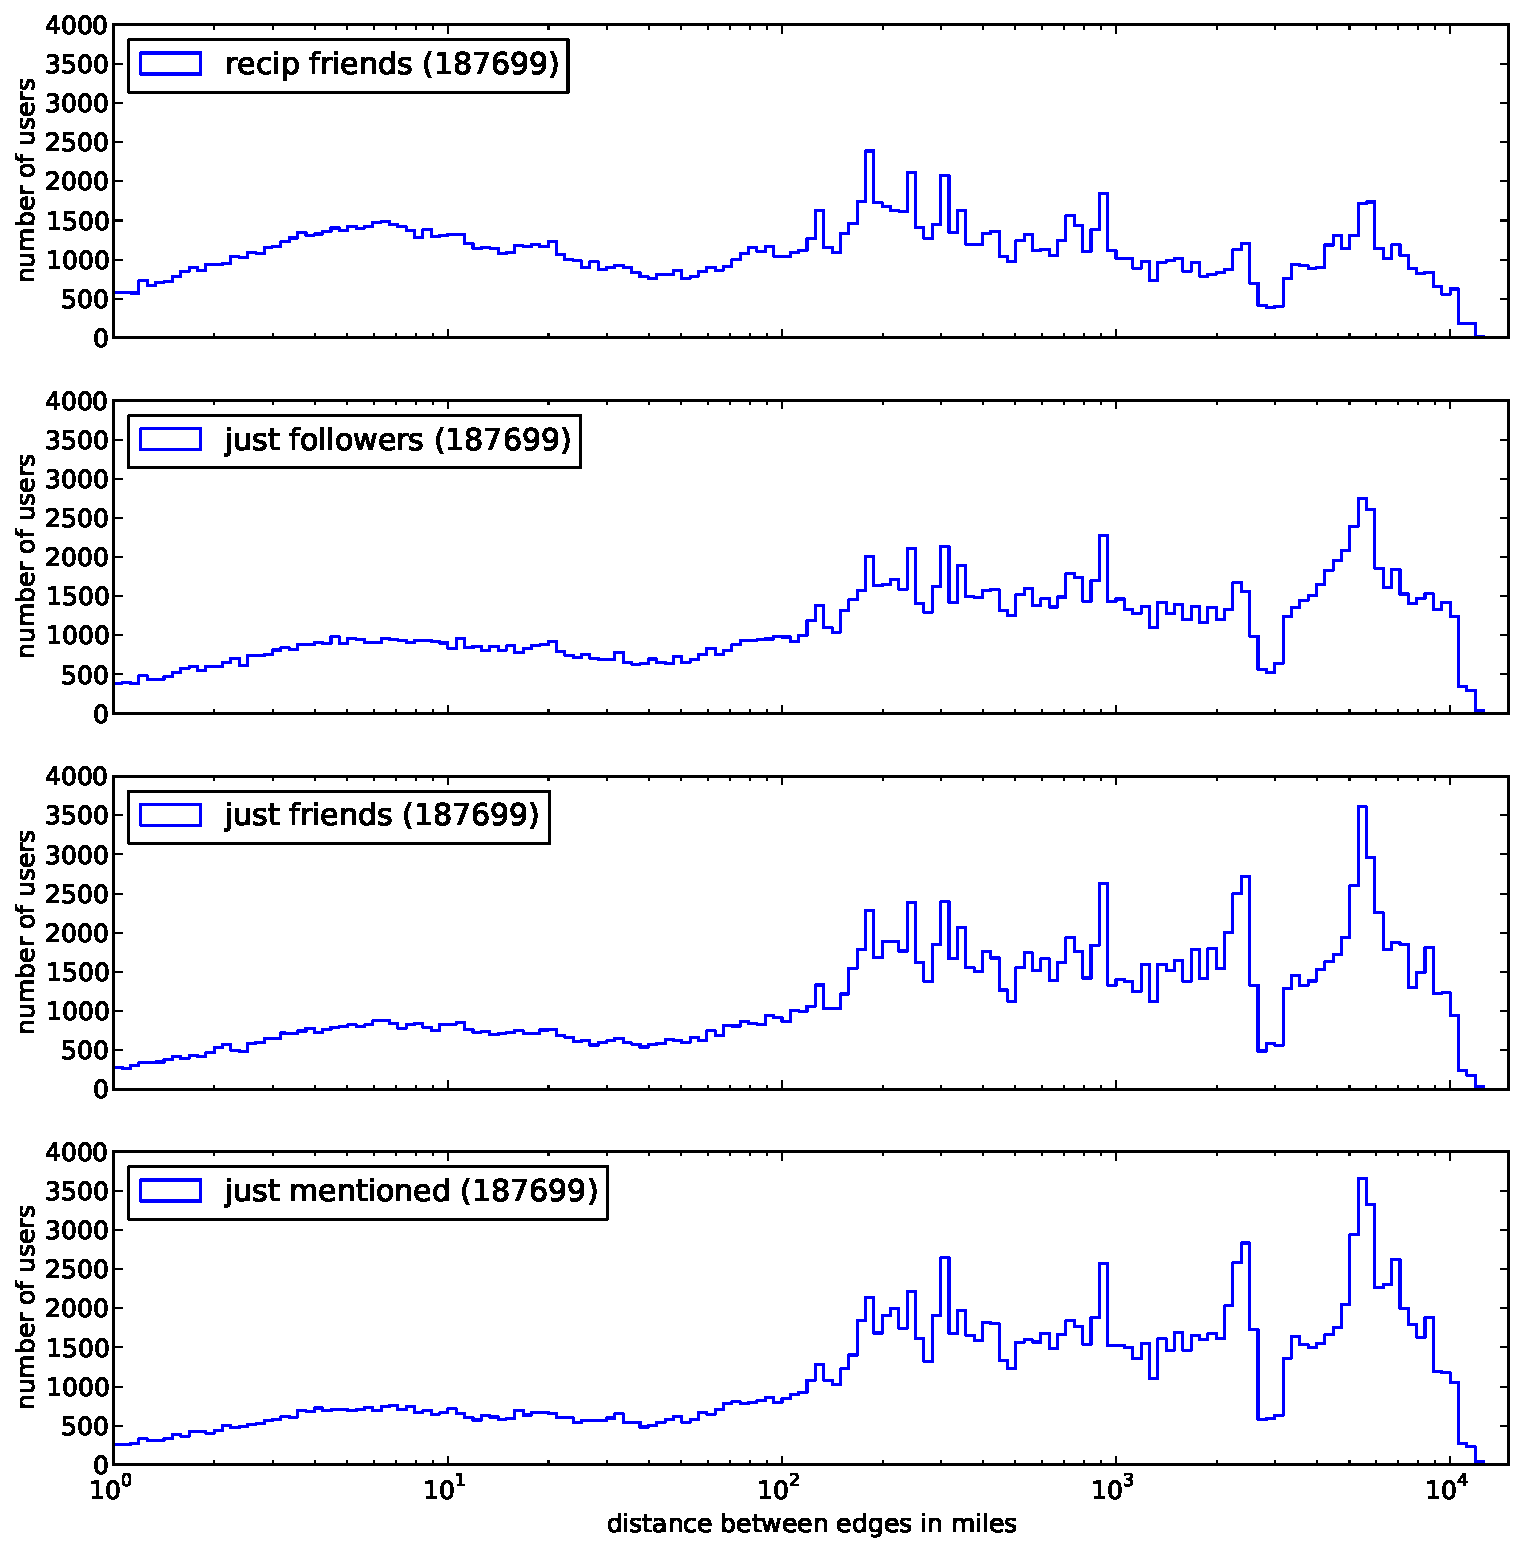
\includegraphics[width=\linewidth]{figures/edge_types_norm.pdf}
\caption{
Histogram of distance to users for different types of relationships.
The curves in this figure are the derivatives of the curves in
Figure~\ref{fig:EdgeTypesCum}.
}
\label{fig:EdgeTypes}
\end{figure}

To understand the distribution of contacts, we created a histogram of the distances between various types of contacts.
We sorted the distances to contacts into 200 logarithmically
scaled bins (40 bins for each power of 10).
Figure~\ref{fig:EdgeTypes} shows the result of plotting the histogram.
%
All four types of contacts follow roughly the same
distribution: one peak around 10 miles from people who live nearby, and several
other peeks between 100 and 10,000 miles. These peeks occur at the distances
between major population centers.

One reasonable explanation for this is that Twitter is not just a social
network; it is also a news distribution network.  This distribution
suggests that users have two types of contacts: people who they met in
real life, and people who they met online or know about via mainstream media.
The former group is useful for predicting location and the latter group is not.
In section~\ref{sec:model}, we use this idea that there are two types of
contacts to build a predictive location model based on social ties.


\section{Are users closer to people they communicate with?}

\begin{figure}[tb]
\centering
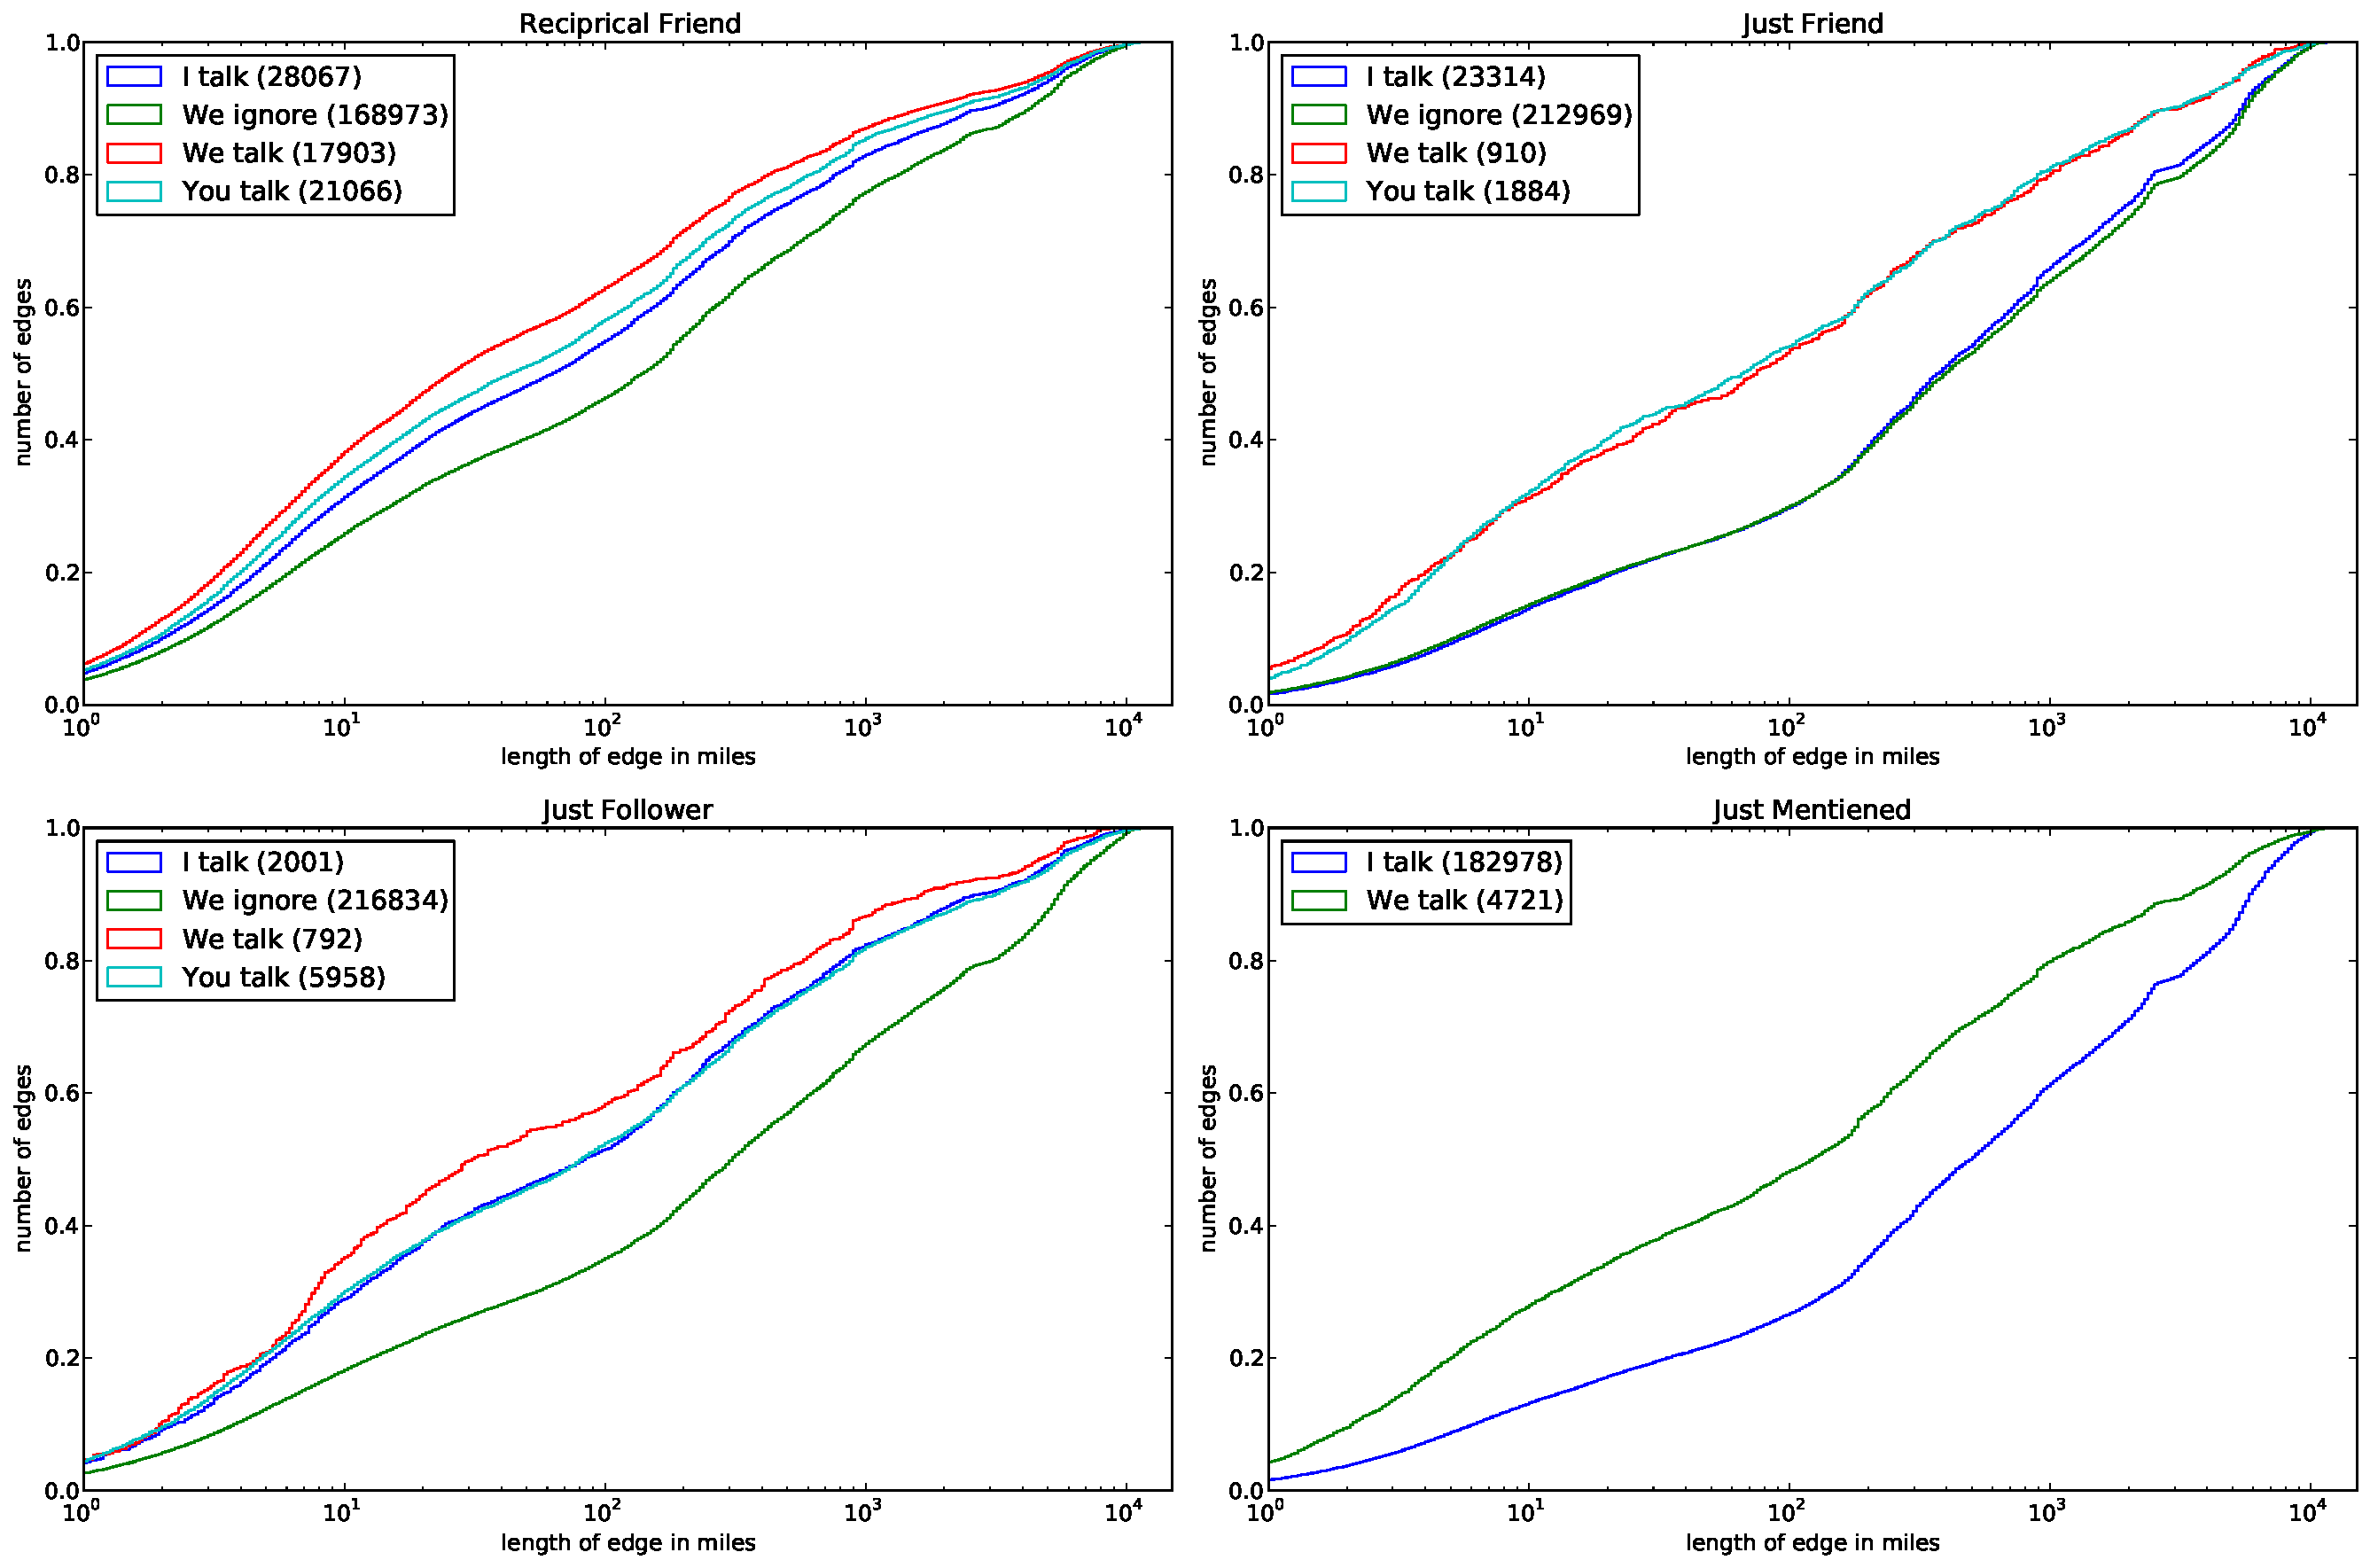
\includegraphics[width=\linewidth]{figures/com_types.pdf}
\caption{
CDF of the distance between a geo-located user and various types of contacts
piloted on a logarithmic scale.
In these graphs, ``I'' refers to the geo-located user. ``You'' refers to their
contact.
}
\label{fig:ComTypes}
\end{figure}

Figure~\ref{fig:ComTypes} shows the relationship between various types of
communication patterns between the geo-located users and their contacts.
In almost every case, increased communication increases the probability that
two users live near each other.
There is one exception: when an average user mentions someone they follow who
does not follow them back, it has no effect.
In other words, if a random user mentions a celebrity who does not bother to
reply, they probably do not live in the same area. This can be seen by the blue
and green lines that are right on top of each other in the Just Friend graph.
On the other hand, in the rare event that someone who is just a friend replies
to their follower, then the probability that they live near each other is much
higher.

The weakest type of contact is for users who were just mentioned, but never
replied to. If the person is mentioned, then 36\% of users with no
friend/follow relationship who have a conversation live within 25 miles.
This is approximately equal to the 35\% of reciprocal friends who ignore each
other and live within 25 miles.
Unsurprisingly, the strongest type of connection is reciprocal friends who
communicate.


\section{Are users closer to private accounts?}

\begin{figure}[tb]
\centering
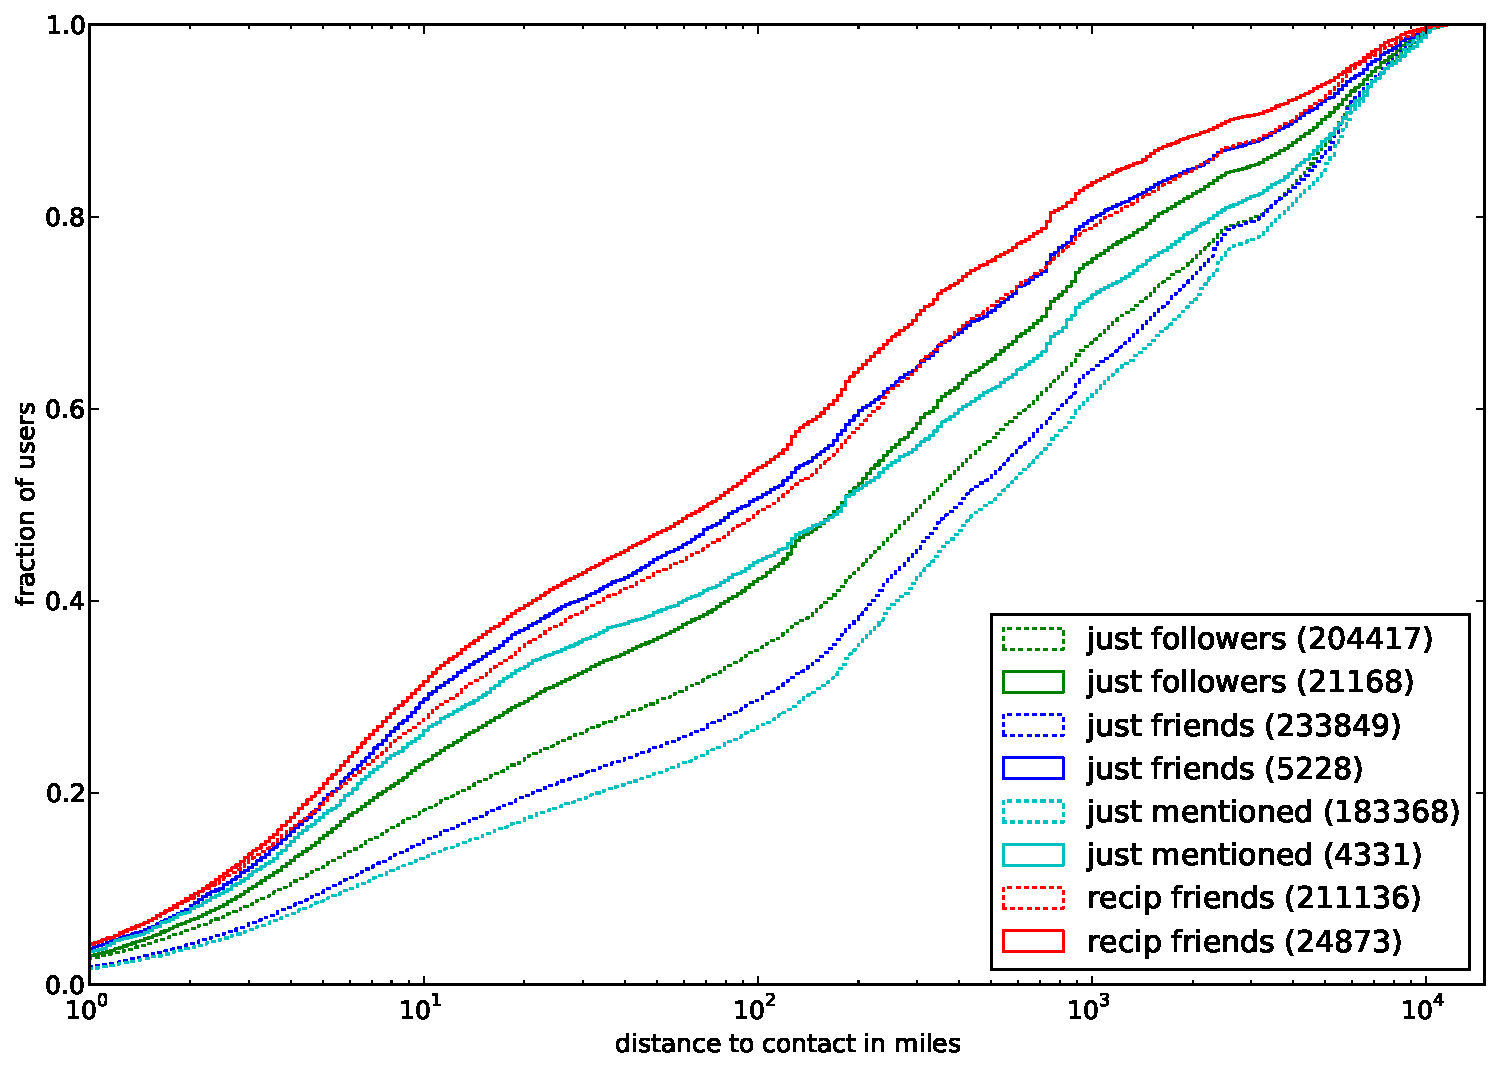
\includegraphics[width=\linewidth]{figures/edge_types_prot.pdf}
\caption{Solid lines represent protected accounts, and dashed lines represent
public accounts. If a user follows a protected account, they tend to be
closer.}
\label{fig:EdgeTypesProt}
\end{figure}

Like many social networks, Twitter allows users to mark their account as
protected. The specifics differ from network to network, but in Twitter's case
a user has to be approved to follow a protected user.
There are demographic differences between public and protected accounts.
For example, Gilbert \cite{gilbert2008network} demonstrates that rural users
are more likely to make their accounts private than public accounts.
In the case of protected accounts on Twitter, basic information
about their profile such as their location and the number of friends and
followers is public, but their friends list, followers list, and the text of
their tweets is private, and not available for analysis.

As seen in figure~\ref{fig:EdgeTypesProt}, the most dramatic difference between
private and public occurs if a user follows a protected account.
%
Since users generally only allow people they know to follow a protected
account, this brings the users almost as close together as if they were
reciprocal friends.
%
On the other hand, if a protected account follows the geo-located user, they
are only slightly more likely to be nearby.

\section{If two of your friends live near each other, does that increase the
chance that they live near you?}

\begin{figure}[tb]
\centering
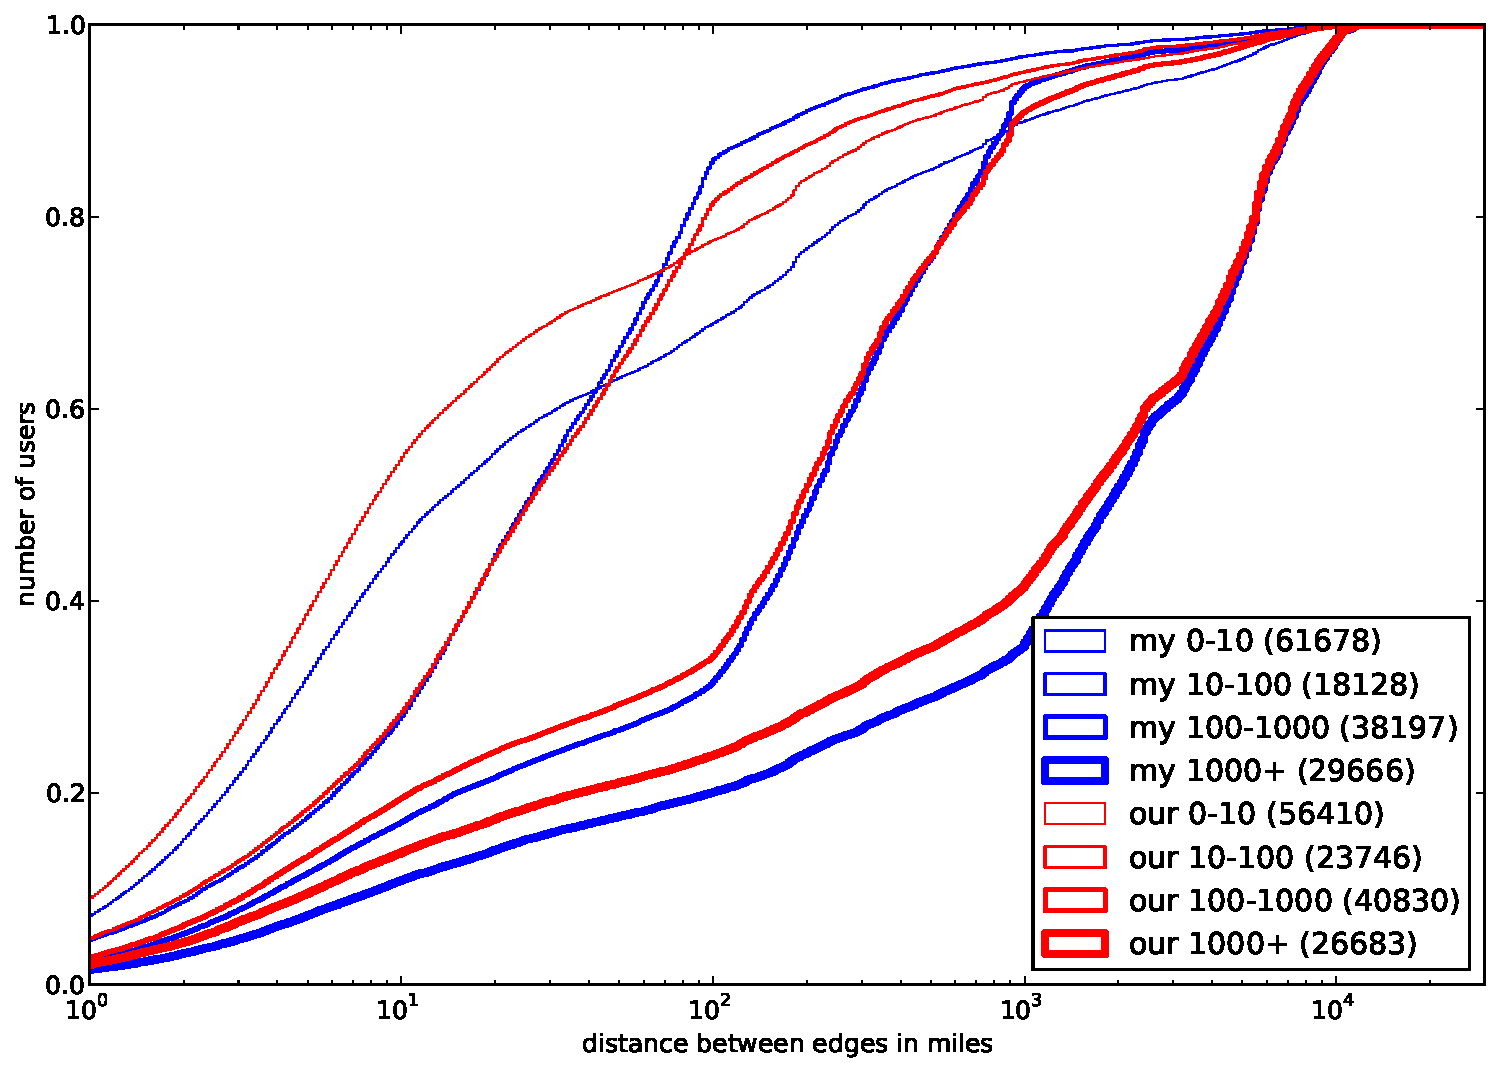
\includegraphics[width=\linewidth]{figures/near_triads.pdf}
\caption{
Comparison between distance to a mutual friend, labeled ``our'', and someone
who is not a mutual friend, labeled ``my''.
The figure in the upper-left corner shows the shape of the social graph we used
to create this graph.
}
\label{fig:NearTriads}
\end{figure}

In this section, we turn our attention to triangles of users.
Finding useful relationships between the edges of a social triangle is tricky
because the three distances depend on each other.
Unfortunately, it is fairly simple to show using the triangle inequality theorem
that if two users are 1000 miles apart, then the third member of the triangle
has to be at least 500 miles from one of the other two.
Since this isn't a useful result, we designed a more complex experiment to
analyze the relationship between the sides of the triangle.
A script searched for a specific pattern in the social network of the
reciprocal friends.  It needed four users who fit the following criteria:
\begin{itemize}
\item ``me'' is the geo-located user
\item ``you'' is reciprocal friends with ``me''
\item ``my'' has no relationship with ``you'' and is reciprocal friends with ``me''
\item ``our'' is reciprocal friends with both ``me'' and ``you''
\end{itemize}

We found this pattern in 147669 of the users in the training set.
If a user had multiple instances of this pattern, it picked one of them
randomly so that particular users would not bias the results.
Since our crawler only retrieved friend and follower information for at most
seven reciprocal friends per user, it is reasonable to assume that this pattern
is much more common, but the sample is more than enough data to draw some
conclusions.

Figure~\ref{fig:NearTriads} shows a comparison between the ``my'' users and the
``our'' users.
For each of the ``my'' users and the ``our'' users, we put them into one of
four logarithmically scaled bins based on their distance from the ``you'' user.
Then we plot the CDF for the distance to ``me'' for each user in the set. This
allows us to investigate the effect of mutual friendship on distance.
We report one very simple result: if two of your friends are close (within 10
miles), then whether they know each other or not is strongly affects how close
you are to them. If they are farther apart, it doesn't matter.

\section{Does the number of friends and followers a person have affect how
close they are?}

\begin{figure}[tb]
\centering
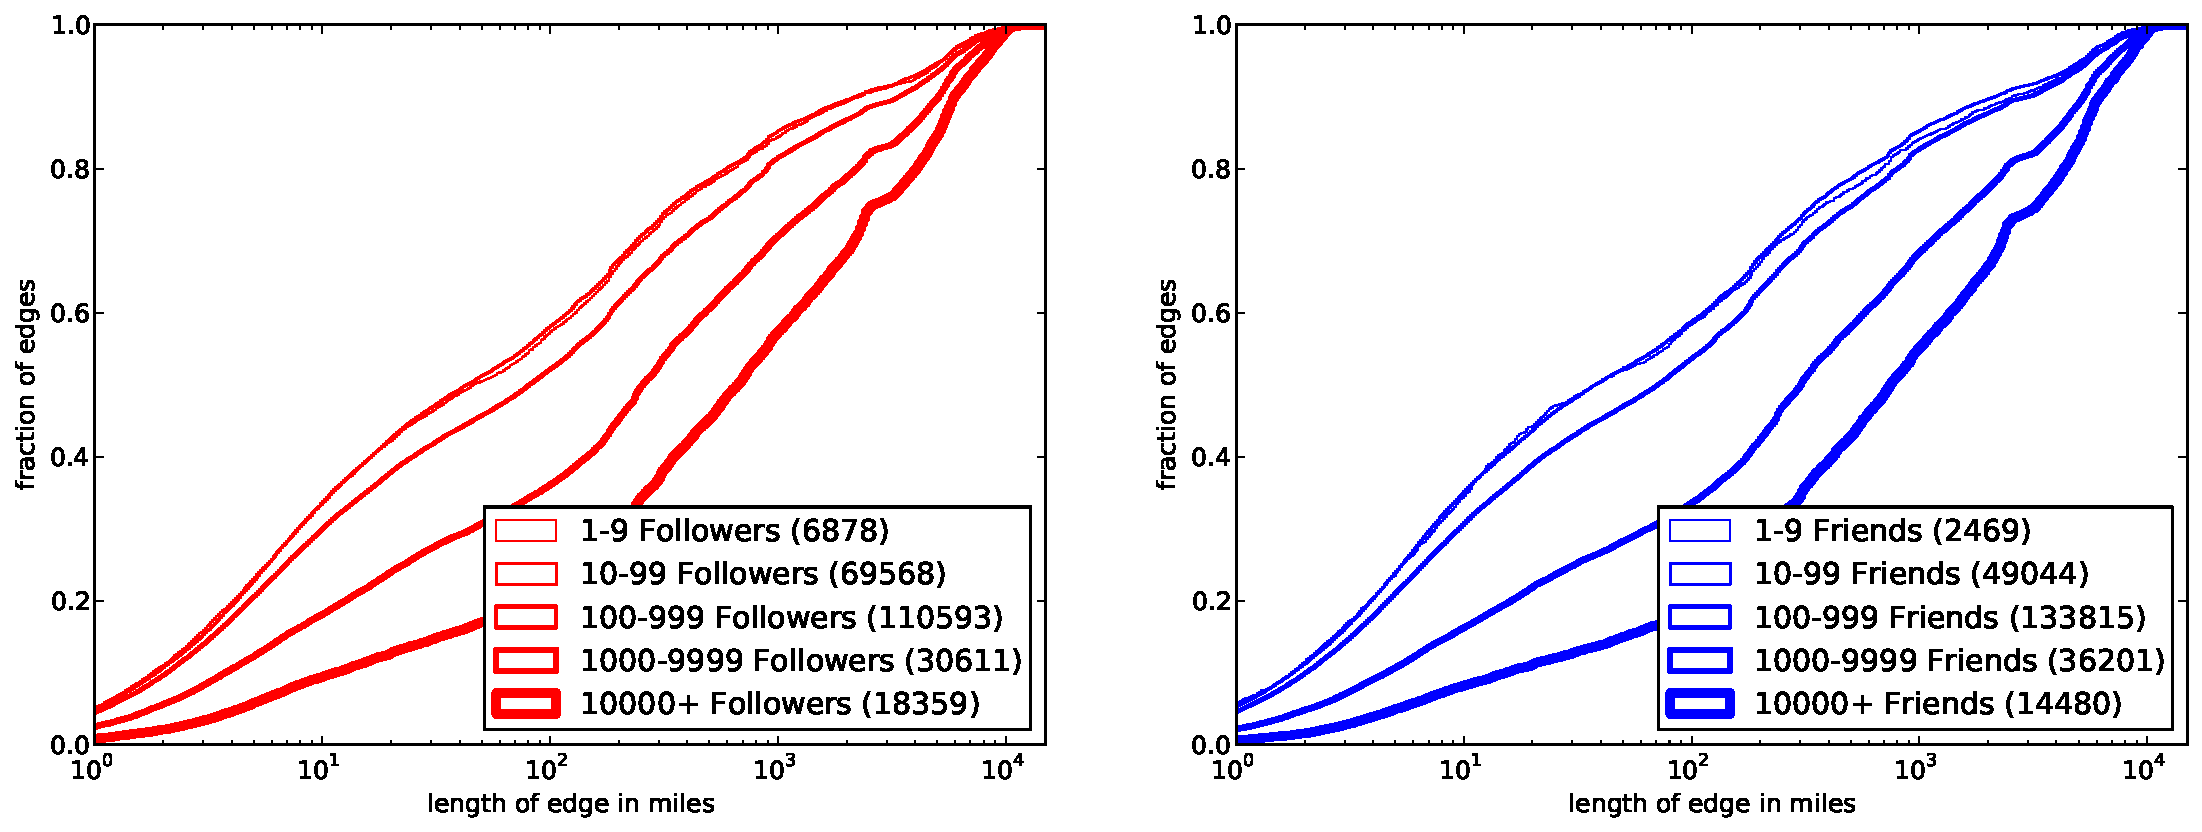
\includegraphics[width=\linewidth]{figures/edge_counts.pdf}
\caption{
A comparison between number of followers and proximity---people who have more
friends or followers tend to be further away.
}
\label{fig:EdgeCounts}
\end{figure}

%FIXME: this is important: should we move it up?

Since the primary goal of this research is to predict the location of users, we
focus our attention on the number of friends and followers a contact has rather
than the numbers for the geo-located user.
We took each of the reciprocal friendships what we looked at in
Section~\ref{sec:EdgeTypes} and put them into log-scaled bins based on their
number of friends or followers that the contact had.
Figure~\ref{fig:EdgeCounts} shows the result of this procedure.

In general, people who are more promiscuous followers and friends are less
likely to live nearby. This makes sense because it is easy to meet 5 Twitter
users in real life, but very few people know 500 Twitter users who live in the
same town.

Mainstream media and celebrity accounts such as the New York Times and Lady
Gaga have millions of followers while normal users rarely have more than a few
hundred.
Follower count is a good way to distinguish celebrity and news accounts which
are useless for location prediction.

\section{Are some users closer to all of their friends and followers?}

\begin{figure}[tb]
\centering
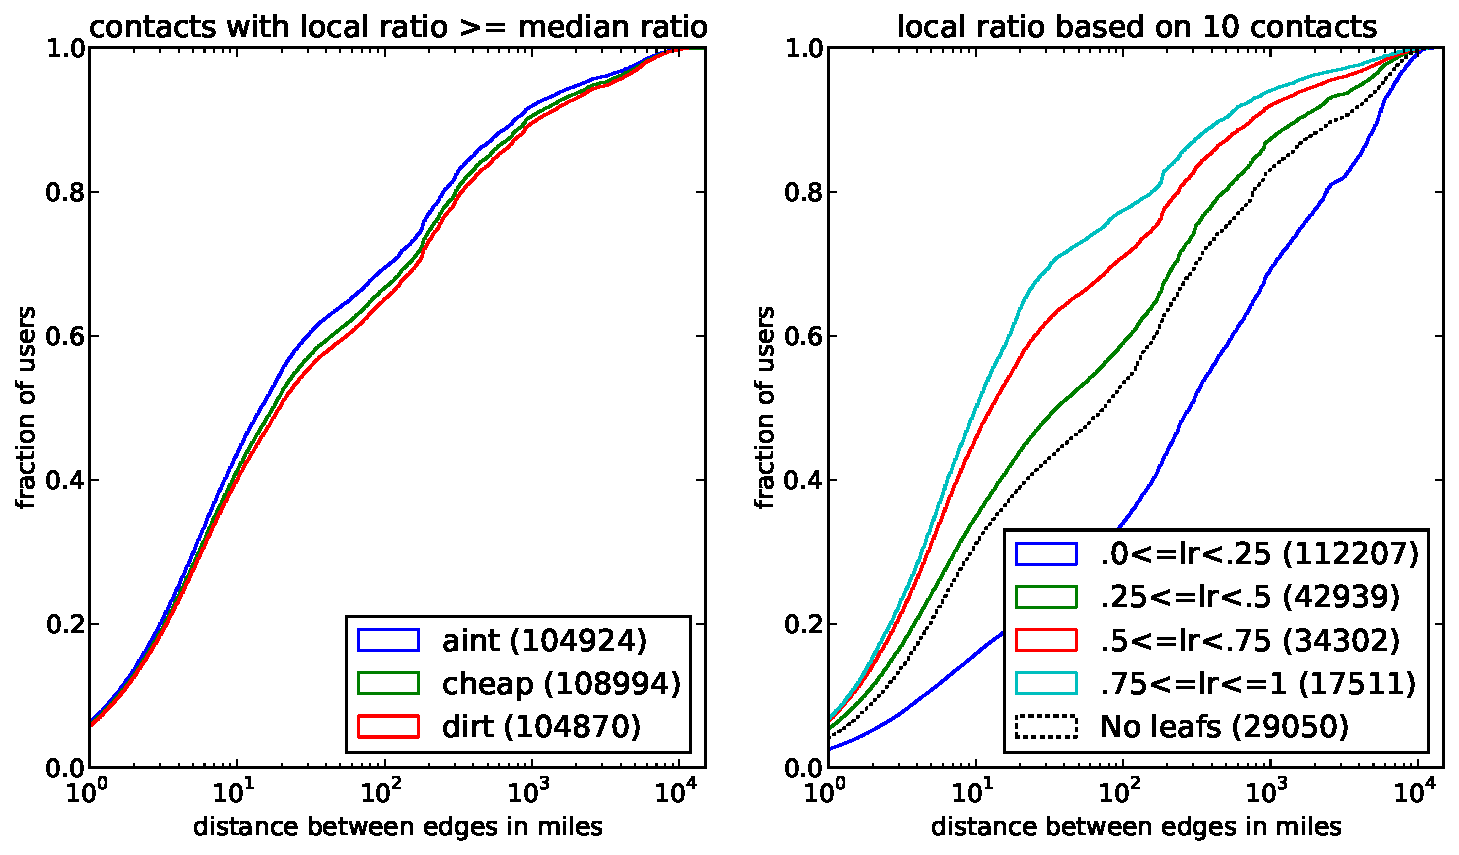
\includegraphics[width=\linewidth]{figures/local_ratio.pdf}
\caption{
The colored lines show the distance to contacts split into groups based on the
proportion of the contact's friends and followers who live near the contact.
The dotted line shows the distance to contacts who have no locatable contacts.
}
\label{fig:LocalRatio}
\end{figure}

In the previous sections we only looked at the contacts of the geo-located
users. In this section we will go two steps out on the social graph and
investigate the friends-of-friends.
%
For each of the contacts we calculated the distance to at most fifty followers.
%
\textbf{Local Contact Ratio} is the fraction of those followers who lived within 25 miles
of the contact.
% FIXME: update this with the new graphs
%
Around one in ten contacts did not have any followers with a location they were
treated as a separate group.
%
We repeated this procedure on the contacts' friends to produce
Figure~\ref{fig:EdgeCounts}.

The figure shows that some users are much more local than other users.
For example, a local newspaper may have thousands of followers and few friends,
but the people who follow a newspaper are generally local.
According to the other factors we looked at, the newspaper is a bad predictor
of location, but in reality it is a great predictor.

Of the factors we have investigated, this is the most strongly correlated with
distance.
One problem with this technique is that it is somewhat expensive to deal with
the profiles two steps out on the social graph.
It may be possible to achieve similar results by visiting fewer
friends-of-friends.

\ifdefined\THESIS
    \chapter{\uppercase{Location Prediction}}
\else
    \section{Location Prediction}
\fi

Based on the questions we answered in the previous section, we have enough
information to build a system for location prediction, which we call
FriendlyLocation.
%
Since the location prediction system will be run on a large number of users,
it must be fast and scalable.
%
In Chapter~\ref{chap:eval} we will evaluate this system using five-fold cross
validation.
%
In this chapter we will use the numbers from one of the five folds to make
the descriptions more concrete.

\section{Edge Length Prediction}

We need to separate the best contacts, who are likely to be nearby, from
bad contacts who are likely to be far away.
%
The factors that we investigated in the previous section indicate when someone
is likely to be nearby, but they don't guarantee it.
%
There are pairs of users who are reciprocal friends with a small number of
followers, a high local friend ratio, have conversations, and still live on
opposite sides of the globe.
%
Another problem with this data is that some of these factors are correlated
with each other; users with lots of followers tend to have a low friend contact
ratio.
%
Finally, distant accounts like celebrities may be useless for determining which
city a person is from, but they might still suggest the user's home continent.

In \cite{backstrom2010find}, the authors present a model of the relationship
between distance and friendship that treats all of the edges the same.
%
We can improve the accuracy of this model by weighting some edges more strongly
than others.
%
We have several pieces of information, and want to map it to a single, extremely
noisy value: the distance to a contact.
%
This could be looked at as a classification problem where you want to classify
edges as local or non-local, but the problem is there is a smooth continuum
from local to non-local, and semi-local friends can be useful for location
prediction.
%
As a result, we model this as a regression problem.
%
Since most of the input features are correlated and either binary or non-linear,
linear regression is unlikely to work well.
%
In addition, the data is dense and low-dimensional, so Support Vector Machines
do not work well.
%
We chose to use a decision tree regressor based on the CART algorithm
(classification and regression trees) to distinguish the best edges from the
worst.
%
A decision tree regressor works similar to the well-known decision tree
classifier, except that it produces real numbers as output instead of discrete
classes.
%
During training, the training data is recursively split based on the input
variable with the most predictive power to build a binary tree.
%
Each of the internal nodes of this tree have a cutoff for one of the input
variables, and the leaves of the tree have a predicted value.
%
\jam{Does this need a better explanation? Can we assume people know decision
trees?}

The regression tree was trained on several of the features from the previous
section that are correlated with users living near each other:
\begin{itemize}
\item the type of contact
\item if the target mentioned the contact
\item if the contact mentioned the target
\item if the contact had a protected account
\item the contact's follower and friend count
\item the PLE of the contact's location
\item the contact's local friend ratio
\end{itemize}
%
Since the distances between users varied by several orders of magnitude, we
trained the regressor to predict the log of the distance.
%
The tree regressor was configured to not split leafs with fewer than 1000 data
points to prevent over-fitting.
%
The top three levels of a decision tree are shown in Figure~\ref{fig:TreeTop}.
%
The predictor does not do a great job of predicting the actual distance to a
contact; there's simply too much noise.
%
However, it does do an excellent job of separating the closest pairs of users
from the most distant pairs as we will show in the next section.

\begin{figure}[tbh]
\centering
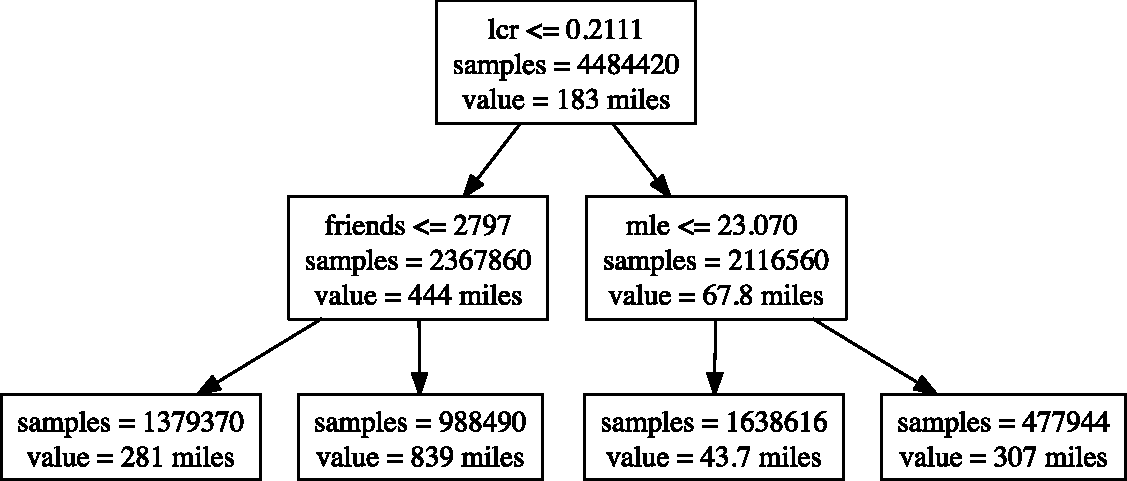
\includegraphics[width=\linewidth]{figures/tree_top.pdf}
\caption{
    The top three levels of the decision tree. This decision tree will predict a
    distance of 839 miles for a contact with a local contact ratio of .2 and
    2800 friends. It will predict a much-closer distance of 43.7 miles for a
    user with a local contact ratio of .5 and a predicted location error of 10
    miles.
}
\label{fig:TreeTop}
\end{figure}

\section{Model}
\label{sec:model}

In the previous sections, we looked at the probability that a contact lives a
certain distance from a given user.
%
In this section, we build a model for the probability that a user, who we refer
to as the target user, lives at a specific location given the approximate
location of his contacts.
%
We will extend the model presented in \cite{backstrom2010find}.
%
Here's how they described their curve for the probability of friendship as a
function of distance:
\begin{quote}
To generate this curve, we aggregate over all individuals, computing the
distance between all $8.1 \times 10^{12}$ pairs of individuals with known
addresses.
We then bucket by intervals of 0.1 miles to compute the total number of pairs
and the number of pairs for which an edge is present, plotting the ratio. It
turns out that we can get a good fit to a curve of the form $a(b+x)^{-c}$.
The exponent very close to $c=-1$ suggests that, at medium to long-range
distances, the probability of friendship is roughly inversely proportional to
distance.
\end{quote}

There are several differences between what they did and what we are doing.
%
First, the data we have is from around the world, so we consider distances up
to 10,000 miles apart instead of stopping at 1,000 miles.
%
The data is a lot noisier in the 1,000--10,000 mile range because of the
distribution of land and oceans on the earth.
%
Next, their dataset had street addresses for approximately 2.9 million
Americans, and they used the friendships between users with street addresses to
do the calculation.
%
Since our geolocated users rarely have connections with other geolocated users
we use the geocoded locations of their contacts, which are less accurate than
street addresses since the locations are usually city names.
%
Finally, the most important difference is that we are not treating all the
edges like they are the same, so we can't fit just one curve.

Location prediction with a maximum likelihood estimator requires an estimate of
the probability that a user lives at a specific location.
%
We can find that probability by comparing the distribution of Twitter users to
the distribution of the contacts.
%
First, we needed a model for the density of Twitter users.
%
We calculate the distance between every target user and every contact
(even for contacts and users who had no relationship).
%
We call the number of target and contact pairs that are $d$ miles apart
$\edges(d)$.

% We aren't doing this anymore.
%In order to speed up this calculation, we divide the world into a $.1$ degree
%by $.1$ degree grid, and count the number of of contacts in each of the spots
%on the grid.
%
%We took the distances between users and sorted them into 360 logarithmically
%scaled bins between 10 miles and 10,000 miles.
%
%(Every edge less than 10 miles was ignored when fitting the curve because it
%was around the size of the grid boxes, and therefore, noisy. Distances greater
%than 10,000 miles are on the opposite side of the world.)
%
%We fit this segment to a power law curve, which gives us a way to estimate
%the distribution of Twitter users.

\jam{curve per leaf}

% i index in R, decision tree tuples
% j index in Q, quantile boundaries
% k index in 

Next, we need to model the probability that two users are contacts.
%
We ran the decision tree regressor on the training data to create a set of
tuples $R = (d^a_i, d^p_i)$ for $d^a_i \in D^a$ and $d^p_i \in D^p$ where
$d^a_i$ is the actual length of the edge, and $d^p_i$ is the value predicted by
the decision tree.
%
We split $R$ into $m$ quantiles on the boundaries $\{q_0,\dots,q_m\}$ as
follows:

\[
    q_j =
    \begin{cases}
        D^p_{(1+\lfloor j|R|/m \rfloor)}, & j=<m \\
        \infty & j=m
    \end{cases}
\]

The quantile for a specific predicted distance $d^p_i$ can be found by
comparing it to the boundaries:
\[
    \quantile(d^p_i) = \max_{j \in \{0,\dots,m\}} \{j: d^p<q_j\}
\]

This lets us find $\contactEdges$, which is the number of users who fit in a
quantile $j$ and had an actual distance of $d$
\[
    \contactEdges(j,d) = |\{
            (d^a_i,d^p_i) \in R :
            d=d^a_i \wedge j=\quantile(d^p_i)
        \}|
\]

By comparing the number of edges that could have existed to the number of edges
that actually exist at a specific distance and in a specific quantile, we can
find the probability that a contact at a specific distance is in a quantile:

\[
\pContact(j,d) = \frac{\contactEdges(j,d)}{\edges(d)}
\]

For each of the quantiles, we can fit $\pContact$ to the curve from
\cite{backstrom2010find}:
\[
    \pContact(j,d) = a_{j} (b_{j}+d)^{-c_{j}}
\]

\begin{figure}[tbh]
\centering
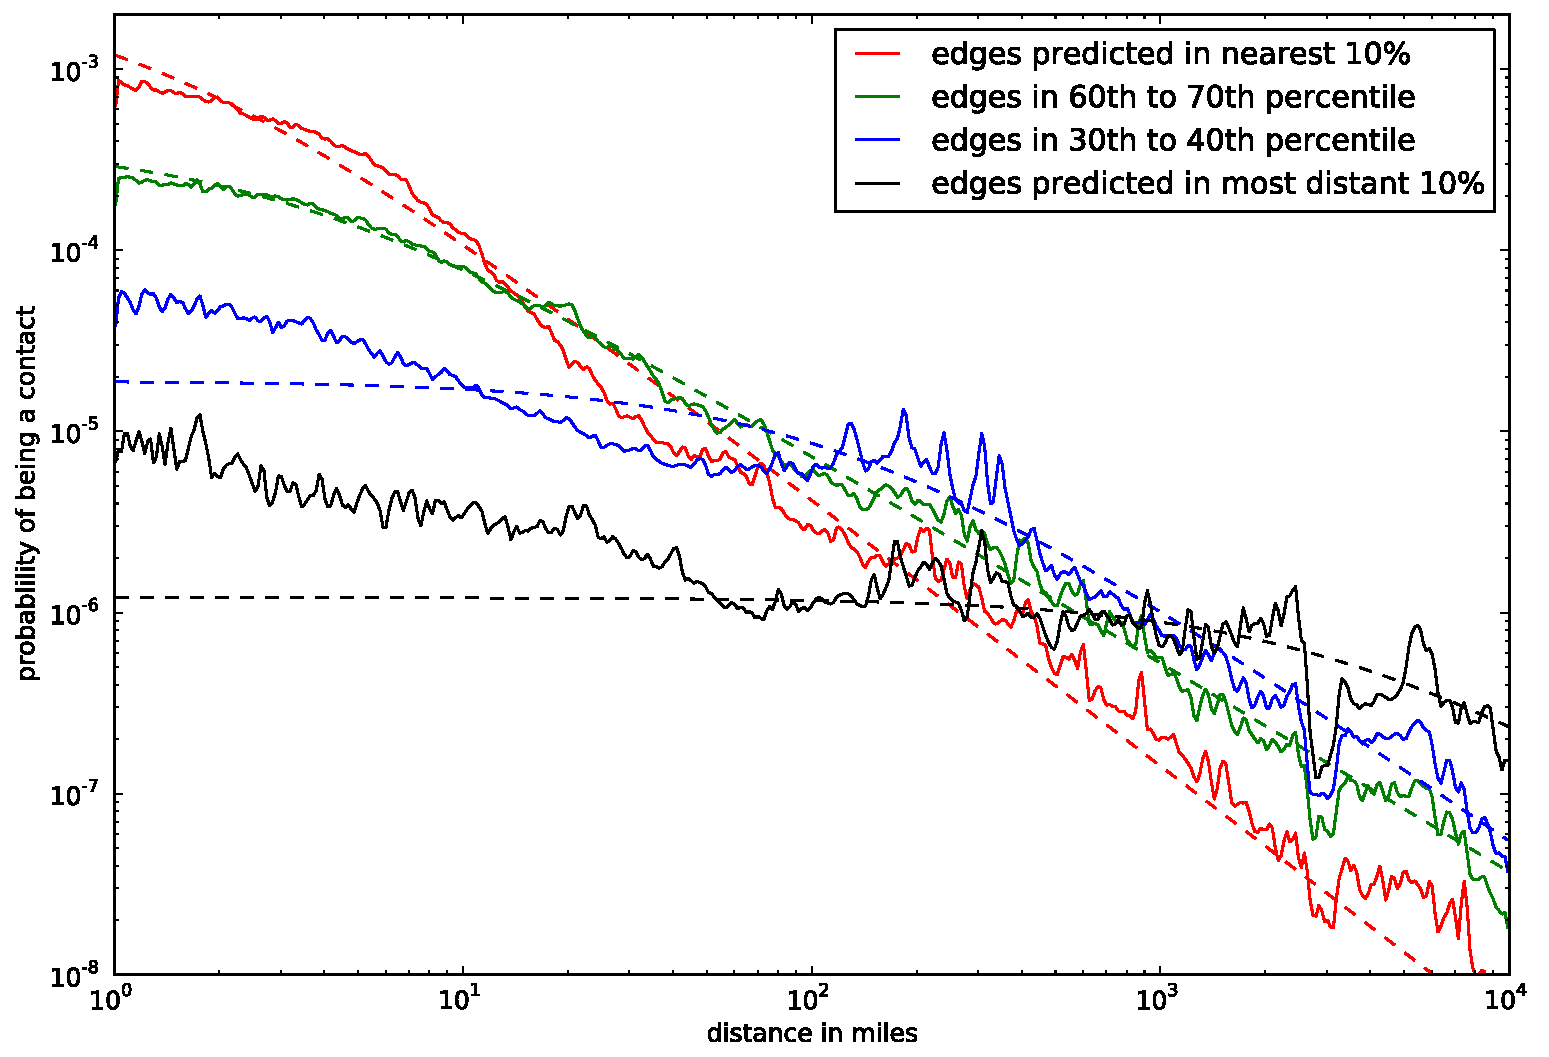
\includegraphics[width=\linewidth]{figures/near_prob_fit.pdf}
\caption{
After splitting edges into groups based on their predicted distance, each group
was fit to a curve. Here are four of the ten curves and their curves of best
fit. The other six curves of best fit are shown as faint dotted lines. The
decision tree does a reasonable job of separating the best edges from the worst
edges.
}
\label{fig:NearProbFit}
\end{figure}

\jam{Why 10? too few - not enough data, too many, just noise}

This gave us 10 different curves for the probability that a certain type of
contact exists between a pair of users.
%
Four of the ten curves from one of the five evaluation groups and their lines
of best fit are shown in Figure~\ref{fig:NearProbFit}.
%
The best contacts are orders of magnitude more
likely to live near a target user than the worst contacts.
%
If the predictions from the tree regressor were ignored, and users were placed
into one group instead of ten equal groups, this would reduce to the model
for friendship and distance presented in \cite{backstrom2010find}.



\section{System}
We used this model to build a maximum-likelihood estimator.

\cite{backstrom2010find}

\jam{cite backstrom:}
\[
    \prod_{(u,v) \in E} p(|l_u-l_v|) \prod_{(u,v) \notin E} 1-p(|l_u-l_v|)
\]

$L^c$ is the set of all contacts
\[
    \pStrangers(l) = \prod_{l^c \in L^c}1-p(|l-l_c|)
\]
pStrangers is shown in Figure~\ref{fig:NearProbFit}.

L is the set of locations of the contacts, and P is the set of predicted
distances for the contacts
\[
    \MLELocation(L,P) = \argmax_{l^c_i \in L}
    \left(
        \pStrangers(l^c_i)
        \prod_{l^c_j \in L,p_j \in P} \pContact(\quantile(p_j),|l^c_i-l^c_j|)
    \right)
\]

\begin{algorithm}
  %\label{alg:friendloc}
  \caption{FriendlyLocation \label{alg:friendloc}}
  \begin{algorithmic}[0]
  \Input{The contacts $contacts$}
  \Output{The predicted location}
  \State locations = list()
  \State predictedDists = list()
  \ForEach{contact \textbf{in} contacts}
      \If{contact.location \textbf{is} None}
        \State \Continue
      \EndIf
      \State locations.append(contact.location)
      \State dist = regressionTree.predict(contact.features)
      \State predictedDists.append(dist)
  \EndFor
  \State best = MLELocation(locations,predictedDists)
  \State \Return locations[best]
  \end{algorithmic}
\end{algorithm}

\jam{formula for MLE, and description,
more here,
non-independent as seen in~\ref{sec:closer}
}

\begin{figure}[tbh]
\centering
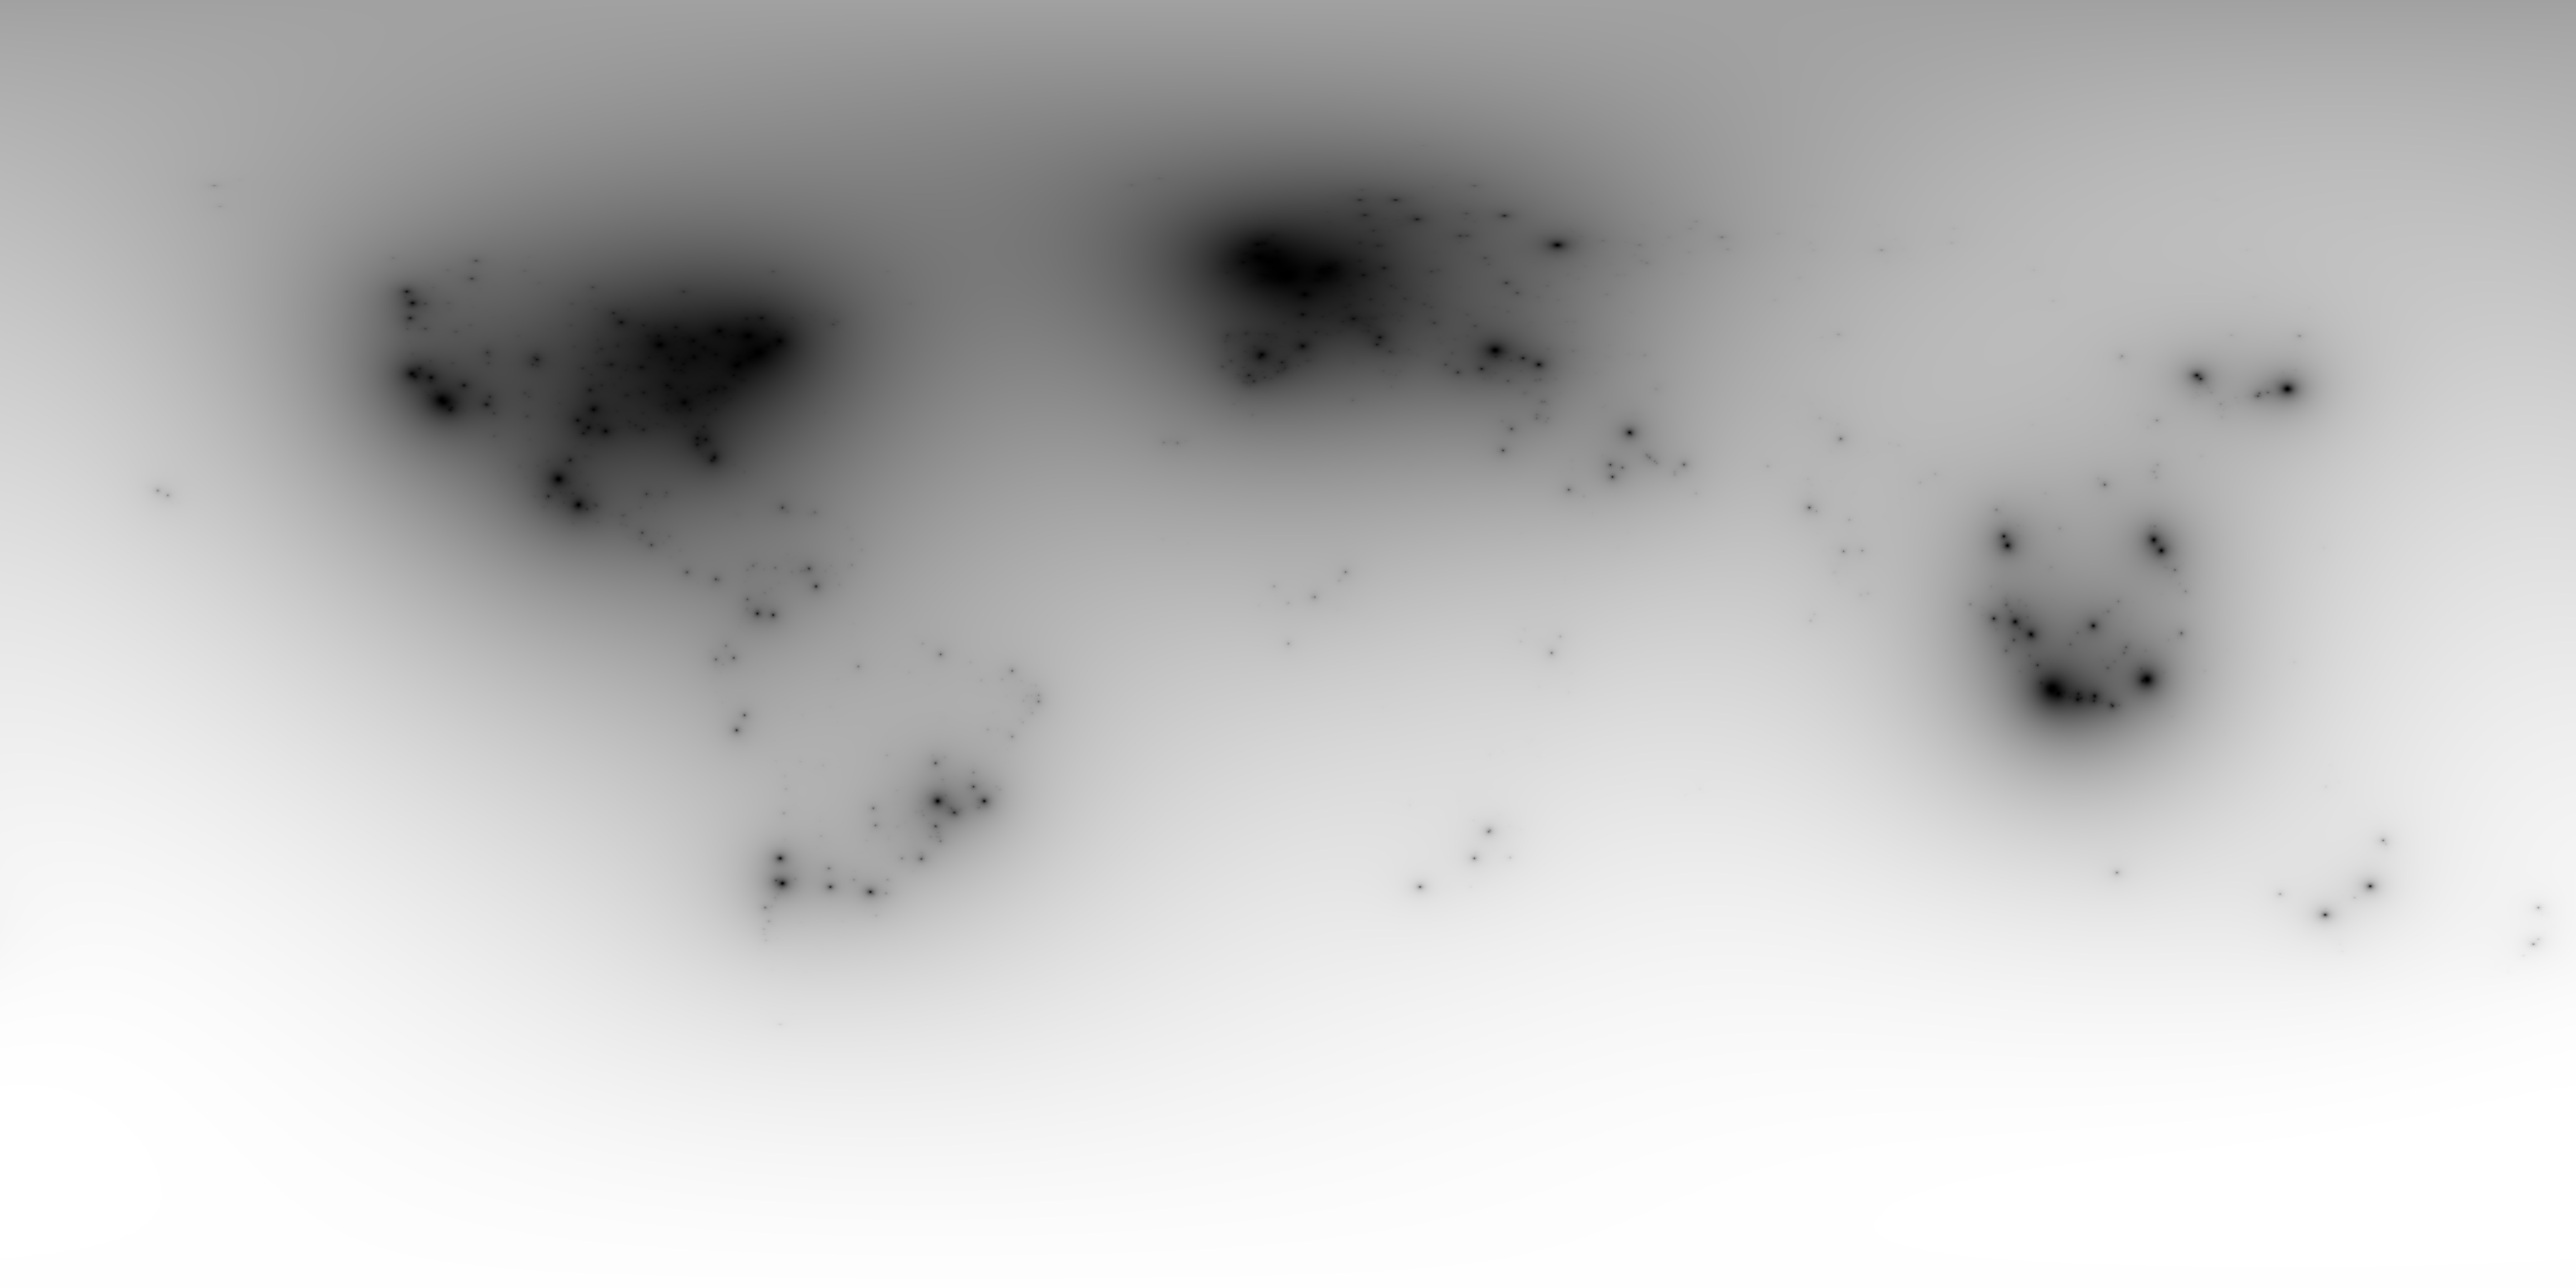
\includegraphics[width=\linewidth]{figures/stranger_mat.png}
\caption{
    This is the probability that a user lives at a location based on the people
    who they have no contact with. Dark areas have lower probability, and light
    areas have a higher probability.
    \jam{blah}
}
\label{fig:StrangerMat}
\end{figure}



\section{Evaluation}
We evaluate the system against several baseline implementations, and evaluate
how the performance of the system varies with the number of contacts a user has
and how many FriendlyLocation chooses to use.

The geo-located users we used to do the evaluation are less concerned about the
privacy of their location information than the average twitter user.
As a result, they tended to give better information in the location field of
their user profile than the average twitter user.
FIXME: we added noise instead
For this evaluation we choose to ignore the contents of the geo-located user's
location fields.
It is likely that better results could be achieved in practice
by using the user's reported location a significant factor in the maximum
likelihood estimation.

We evaluated the FriendlyLocation system against FIXME of the FIXME users from
the evaluation group.
FIXME users from this set were removed because none of their friends or
followers had decodable locations.
(When the crawler initially created the evaluation set it filtered out users
with both zero friends and zero followers.)

We investigate several implementations of the FriendlyLocation system:
\begin{description}
\item[Simple] This system treats all contacts equally---it ignores their
predicted location error and any information about what type of contact it is.
Users are selected randomly and it uses the same parameters for all the users.
\item[Location Error] This shows the value of calculating the median location
error. Users are selected randomly.
\item[Relationship Types] This shows the value of treating contacts differently
based on the type of contact.
Users who are more likely to live near the target user, such as reciprocal
friends, are chosen first.
\item[Full] This is the system described in the previous section. It selects
users based on relationship type, uses the parameters from the training, and
uses predicted location error to evaluate the quality of the contact.
\item[FIXME] Add some more here
\end{description}

In addition to using the FriendlyLocation system as described in the previous
section, we created a few baseline location predictors:
\begin{description}
\item[Median] Finds the median of the latitude and the median of the longitude
of 100 randomly selected contacts.
\item[Mode] Finds the most common location of 100 randomly selected contacts,
and breaks ties by picking one randomly.
\item[Backstrom] FIXME
\item[Omniscient] Finds the contact that is closest to the user from 100 users
selected by the same method used in the Full system.
\end{description}

FIXME: the rest of this section is mostly wrong

Figure~\ref{fig:FinalResults} shows a comparison to the results from the 
different predictors.
Our Full FriendlyLocation system predicts the location within 25 miles FIXME\% of
the time.
Unfortunately, when the predictor system is wrong, it can be very wrong; often
when it would pick not just the wrong city, but the wrong side of the
country.
Both using location error and relationship type improved the predictor.  The
simplified version of FriendlyLocation located users within 25 miles 54\% of
the time which is still better than the either of the baseline predictors.
The omniscient predictor demonstrates that there is still room for improvement
which we discuss in the final section.

We investigated the effect of increasing numbers of contacts on the quality of
the results.
Before removing contacts without location information, we sorted the users into
groups based on the number of contacts the had.
Next, we ran the FriendlyLocation predictor against each of them.
Figure~\ref{fig:LulResults} shows the results of prediction.
The quality of the results from the predictor was lower for users with fewer
than 50 contacts; however, as contacts increased beyond that, it had no
significant effect on the results.


The final step of the evaluation is to investigate if FriendlyLocation would
work with a smaller number of profiles than 100.
For all of the users with more than 200 contacts, we sorted their contacts in
order of decreasing probability that they were local.
Then we ran FriendlyLocation on the top \(n\) contacts for
\(n\in (5,10,15,25,100)\).
The results shown in Figure~\ref{fig:TopResults} for 25 contacts are almost as
good as the results for 100 contacts. This means that our algorithm only needs
location information for around ten users to make reasonable predictions.




\flchap{Conclusion}
We demonstrated that some types of relationships tend to be closer than others,
identified some features of relationships that are correlated with physical
proximity, and used this to accurately predict the locations of users on a
social media website.
There are two directions that the future work on this project could go:
improving the results of the predictor and using the predicted locations in
other research projects.

\emph{Do you talk about future work in a thesis?}

One way to improve this predictor is to combine tie strength and the social
graph with other factors such as the words users choose to use as described by
Cheng \cite{cheng2010you}.
It could be useful for the predictor to return not just a location, but an
estimate of the quality of the prediction.  This paper only considered
users who have a well-defined location. FriendlyLocation could identify users
who do not have meaningful locations such as people who constantly travel.
This could work well with the node locality metric which is defined by
Scellato\cite{scellato2010distance}.

Finally, high-quality geographic information opens up new avenues for research.
With geographic location of users, we can cluster users and find local
conversations.
It also allows businesses to provide hyper-local content and services.




%%%%%%%%%%%%%%%%%%%%%%%%%%%%%%%%%%%%%%%%%%%%%%%%%%%
%
%  New template code for TAMU Theses and Dissertations starting Fall 2012.  
%  For more info about this template or the 
%  TAMU LaTeX User's Group, see http://www.howdy.me/.
%
%  Author: Wendy Lynn Turner 
%	 Version 1.0 
%  Last updated 8/5/2012
%
%%%%%%%%%%%%%%%%%%%%%%%%%%%%%%%%%%%%%%%%%%%%%%%%%%%


%%%%%%%%%%%%%%%%%%%%%%%%%%%%%%%%%%%%%%%%%%%%%%%%%%%%%%%%%%%%%%%%%%%%%%
%%                           REFERENCES 
%%%%%%%%%%%%%%%%%%%%%%%%%%%%%%%%%%%%%%%%%%%%%%%%%%%%%%%%%%%%%%%%%%%%%

\phantomsection
\addcontentsline{toc}{chapter}{REFERENCES}

\renewcommand{\bibname}{{\normalsize\rm REFERENCES}}

\bibliographystyle{plain}
\bibliography{fl}

%%%%%%%%%%%%%%%%%%%%%%%%%%%%%%%%%%%%%%%%%%%%%%%%%%%%
%
%  New template code for TAMU Theses and Dissertations starting Fall 2012.  
%  For more info about this template or the 
%  TAMU LaTeX User's Group, see http://www.howdy.me/.
%
%  Author: Wendy Lynn Turner 
%	 Version 1.0 
%  Last updated 8/5/2012
%
%%%%%%%%%%%%%%%%%%%%%%%%%%%%%%%%%%%%%%%%%%%%%%%%%%%

\begin{appendices}
\titleformat{\chapter}{\centering\normalsize}{APPENDIX \thechapter}{0em}{\vskip .5\baselineskip\centering}
\renewcommand{\appendixname}{APPENDIX}

%%%%%%%%%%%%%%%%%%%%%%%%%%%%%%%%%%%%%%%%%%%%%%%%%%%
%
%  New template code for TAMU Theses and Dissertations starting Fall 2012.  
%  For more info about this template or the 
%  TAMU LaTeX User's Group, see http://www.howdy.me/.
%
%  Author: Wendy Lynn Turner 
%	 Version 1.0 
%  Last updated 8/5/2012
%
%%%%%%%%%%%%%%%%%%%%%%%%%%%%%%%%%%%%%%%%%%%%%%%%%%%

%%%%%%%%%%%%%%%%%%%%%%%%%%%%%%%%%%%%%%%%%%%%%%%%%%%%%%%%%%%%%%%%%%%%%%
%%                           APPENDIX A 
%%%%%%%%%%%%%%%%%%%%%%%%%%%%%%%%%%%%%%%%%%%%%%%%%%%%%%%%%%%%%%%%%%%%%

\phantomsection

\chapter{\uppercase{First Appendix}}

Text for the Appendix follows.

\begin{figure}[H]
\centering
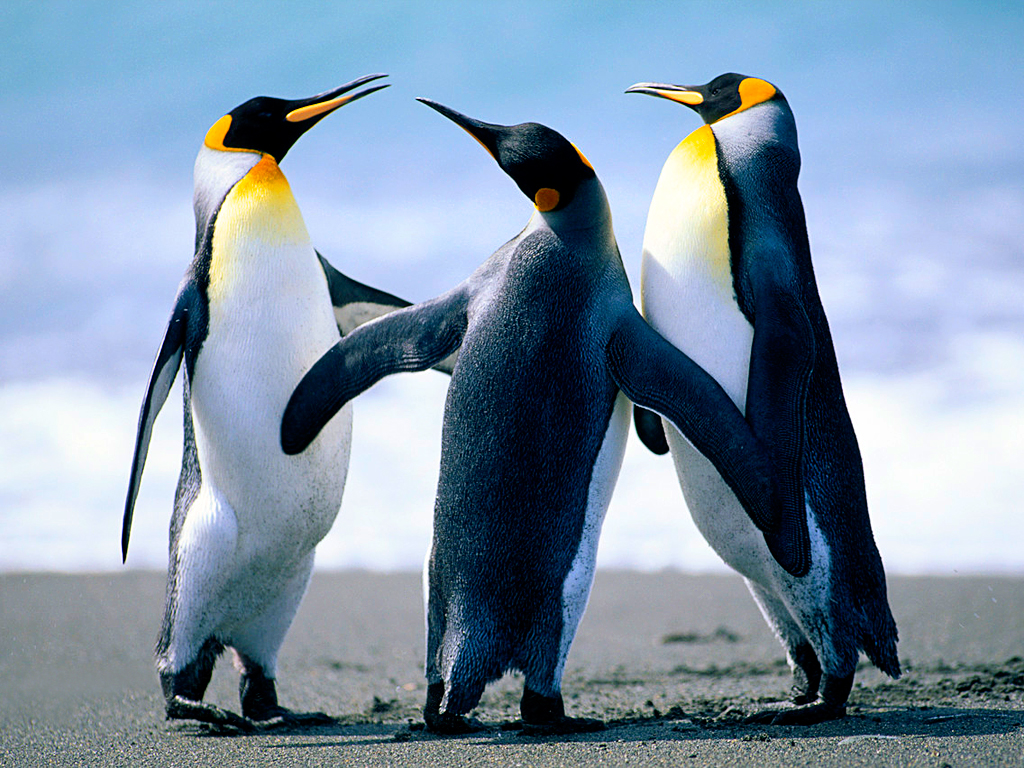
\includegraphics[scale=.50]{figures/Penguins.jpg}
\caption{TAMU figure}
\label{fig:tamu-fig5}
\end{figure}

%%%%%%%%%%%%%%%%%%%%%%%%%%%%%%%%%%%%%%%%%%%%%%%%%%%
%
%  New template code for TAMU Theses and Dissertations starting Fall 2012.  
%  For more info about this template or the 
%  TAMU LaTeX User's Group, see http://www.howdy.me/.
%
%  Author: Wendy Lynn Turner 
%	 Version 1.0 
%  Last updated 8/5/2012
%
%%%%%%%%%%%%%%%%%%%%%%%%%%%%%%%%%%%%%%%%%%%%%%%%%%%

%%%%%%%%%%%%%%%%%%%%%%%%%%%%%%%%%%%%%%%%%%%%%%%%%%%%%%%%%%%%%%%%%%%%%%
%%                           APPENDIX B
%%%%%%%%%%%%%%%%%%%%%%%%%%%%%%%%%%%%%%%%%%%%%%%%%%%%%%%%%%%%%%%%%%%%%

\chapter{\uppercase {Second Appendix with a longer title - much longer in fact}}

Text for the Appendix follows.

\begin{figure}[H]
\centering
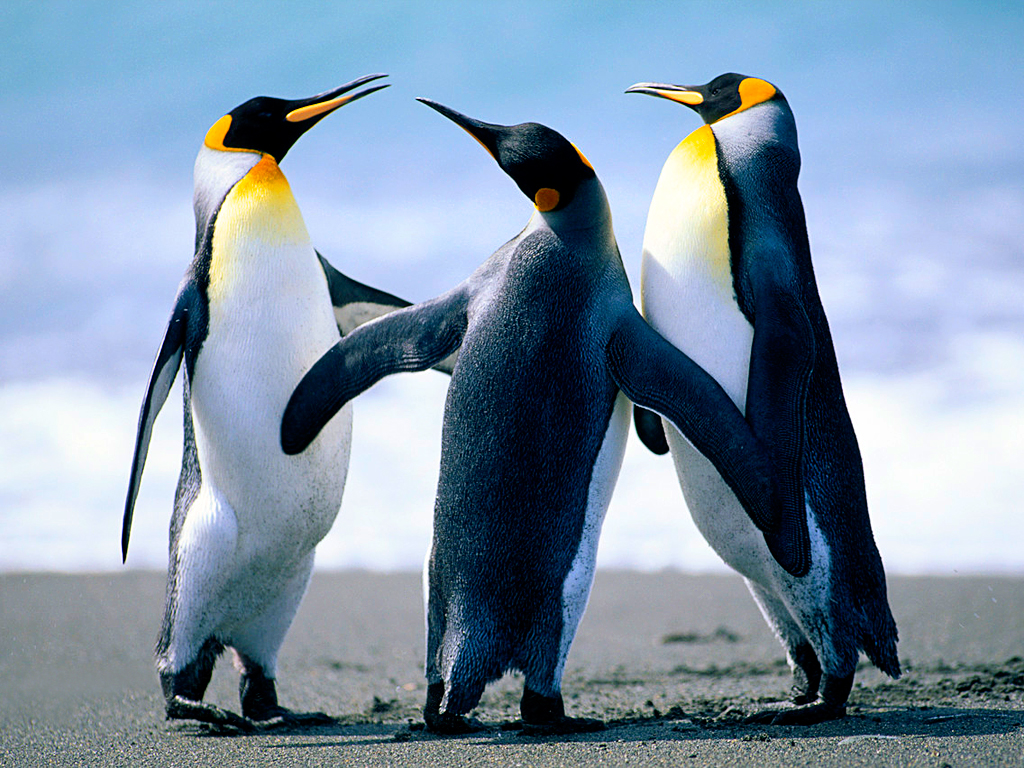
\includegraphics[scale=.50]{figures/Penguins.jpg}
\caption{TAMU figure}
\label{fig:tamu-fig6}
\end{figure}

\section{Appendix Section}


\pagebreak{}

\end{appendices}


\end{document}
